%*******************************************************************************AAA
%*********************************** Chapter XXXXXXXX *****************************
%*******************************************************************************

\nomenclature[z-PoCA]{PoCA}{Point of Closest Approach} 

\chapter{Simulations of the DUNE Far Detector} \label{chap:FDSims} %Title of chapter
\graphicspath{{FarDetectorSimulations/Figs/Raster/}{FarDetectorSimulations/Figs/PDF/}{FarDetectorSimulations/Figs/Vector/}}

Work presented in Chapters~\ref{chap:Cameras},~\ref{chap:35tonSim} and~\ref{chap:35tonData} concerned the 35 ton prototype, however the following simulations have been performed with respect to the DUNE Far Detector (FD). Simulations in the FD have concentrated on cosmogenic background to neutrino oscillations, discussed in Section~\ref{sec:LBNESurf}, and the muon background to nucleon decay, discussed in Section~\ref{sec:DUNENDK}. The simulations shown in Section~\ref{sec:LBNESurf} are discussed in~\citep{MartinsThesis}, and were performed for the Long Baseline Neutrino Experiment (LBNE), which along with the Long Baseline Neutrino Observatory (LBNO), formed the basis for DUNE, and so are included here for completeness. The author contributed by incorporating the \emph{complex} detector geometry, and the accurate surface profile into the simulations, though the main body of work was performed by the author of~\citep{MartinsThesis}. The other work presented was performed for the DUNE collaboration, in conjunction with work done by Vitaly Kudryavtsev and Matthew Robinson, both at the University of Sheffield. This work was performed with the aim of assessing the muon-induced background to nucleon decay in the DUNE FD. \\

%********************************** %Second Section  **************************************
\section{Simulations of the LBNE surface detector} \label{sec:LBNESurf} %Section - X.2
A preliminary design of the LBNE experiment had a 10 kt LAr detector on the surface, with a 3 m rock overburden~\citep{LBNE6493}. Due to the large flux of cosmic rays at such a shallow depth, and the relative scarcity of neutrino events, it is necessary to establish whether the cosmic background can be sufficiently removed to allow neutrino interactions to be discerned. In order to show this, a series of simulations using both a simplified, and a more detailed detector design are performed. The cosmogenic backgrounds due to muons, protons and neutrons, are considered. These simulations, unlike other work presented in this thesis, were performed using a stand-alone version of GEANT4, and not in LArSoft. For a more thorough review of the simulations, see~\citep{MartinsThesis}. \\

Simulations have been built using GEANT4 versions 9.4 and 9.6. Initial simulations were performed using version 9.4, before being rebuilt to use version 9.6. A study showing that the background rate did not change with the newer version of GEANT4 was performed. In all simulations the physics list ``Shielding'' was used~\citep{Shielding}. Shielding allows particles to undergo Compton scattering, inelastic scattering with nuclei and nucleons, and includes all electromagnetic (EM) processes for all leptons, mesons baryons, and generic ions. Muons are able to undergo electron/positron pair production, and electron/positron annihilation is also possible. \\

The authors work built on initial simulations which were performed using a simplified geometry, referred to as the \emph{simple} geometry, which consisted of a single box of LAr measuring 30 $\times$ 15 $\times$ 16 m$^3$. This detector was enclosed in rock measuring (5 $\times$ 10$^3$) $\times$ (5 $\times$ 10$^3$) $\times$ 22 m$^{3}$, in the $x$, $y$, and $z$ coordinates respectively. The detector was positioned so as to have a 3 m overburden of rock. As simulations were not performed in LArSoft, the co-ordinate system used was defined as follows;
\begin{itemize}
\item $x$ - parallel to the beam direction.
\item $y$ - perpendicular to the beam direction.
\item $z$ - vertical direction.
\item The co-ordinate system is centred on the middle of the detector volume in $x$ and $y$, and on the surface of the rock which was above the detector in $z$.
\end{itemize}
The results of these initial simulations, discussed in detail in~\citep{MartinsThesis}, are not shown here, but will be summarised in Table~\ref{tab:SimpSurfRates}. \\

The improvements which the author made to these initial simulations were two fold. Firstly a more detailed geometry, referred to as the \emph{complex} geometry, was included, this had a much more realistic detector design~\citep{LBNE3383}. The \emph{complex} geometry had two identical cryostats, each containing 120 TPC cells measuring 2.52 $\times$ 2.28 $\times$ 7.00 m$^3$. These cells each contain an active volume of LAr measuring 2.27 $\times$ 2.25 $\times$ 6.30 m$^3$. The TPC cells are arranged such that are 10, 6 and 2 TPC cells in the $x$, $y$ and $z$ directions, respectively. This gives a total volume of LAr in each cryostat measuring 28.20 $\times$ 13.95 $\times$ 15.0 m$^3$, with a mass of 5.35 kton. This gives a total fiducial mass of 10.7 kton of active LAr in the two cryostats. Running vertically between the TPC cells are anode plane assemblies (APAs) and cathode plane assemblies (CPA's), all of which are embedded within the larger blocks of LAr. These blocks of LAr are further housed inside stainless steel containers, which are insulated by $0.8$ m of polyurethane. The two cryostats are surrounded by $0.5$ m of concrete on all sides, with $3$ m of concrete separating them. A representation of the detector, produced by the GEANT4 visualisation tool, is shown in Figure~\ref{fig:SurfCompGeom}. \\

%\begin{figure}
%  \centering
%  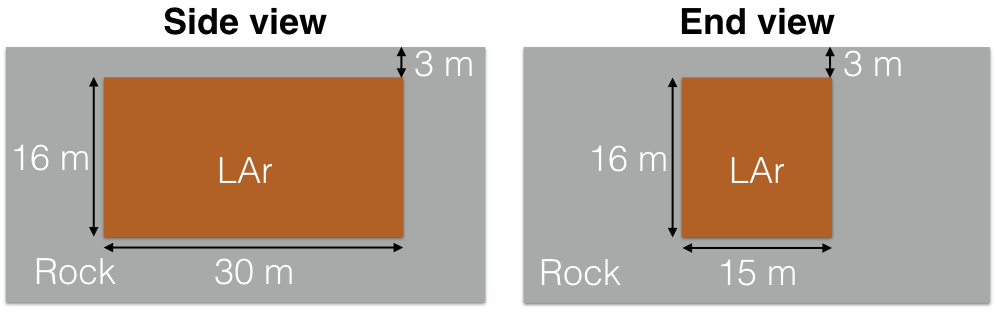
\includegraphics[width=\textwidth]{SimpleDetector}
%  \caption[The \emph{simple} detector geometry used in the LBNE surface detector simulations]
%          {The \emph{simple} detector geometry used in the LBNE surface detector simulations. Both a side view, and an end view are shown to scale. The rock is shown as a grey box. The active volume of LAr is shown as an orange box. The dimensions of the detector, and the overburden are shown in white around the active volume of LAr. Figure is modified from one shown in~\citep{MartinsThesis}.}
%  \label{fig:SurfSimpGeom}
%\end{figure}

\begin{figure}
  \centering
  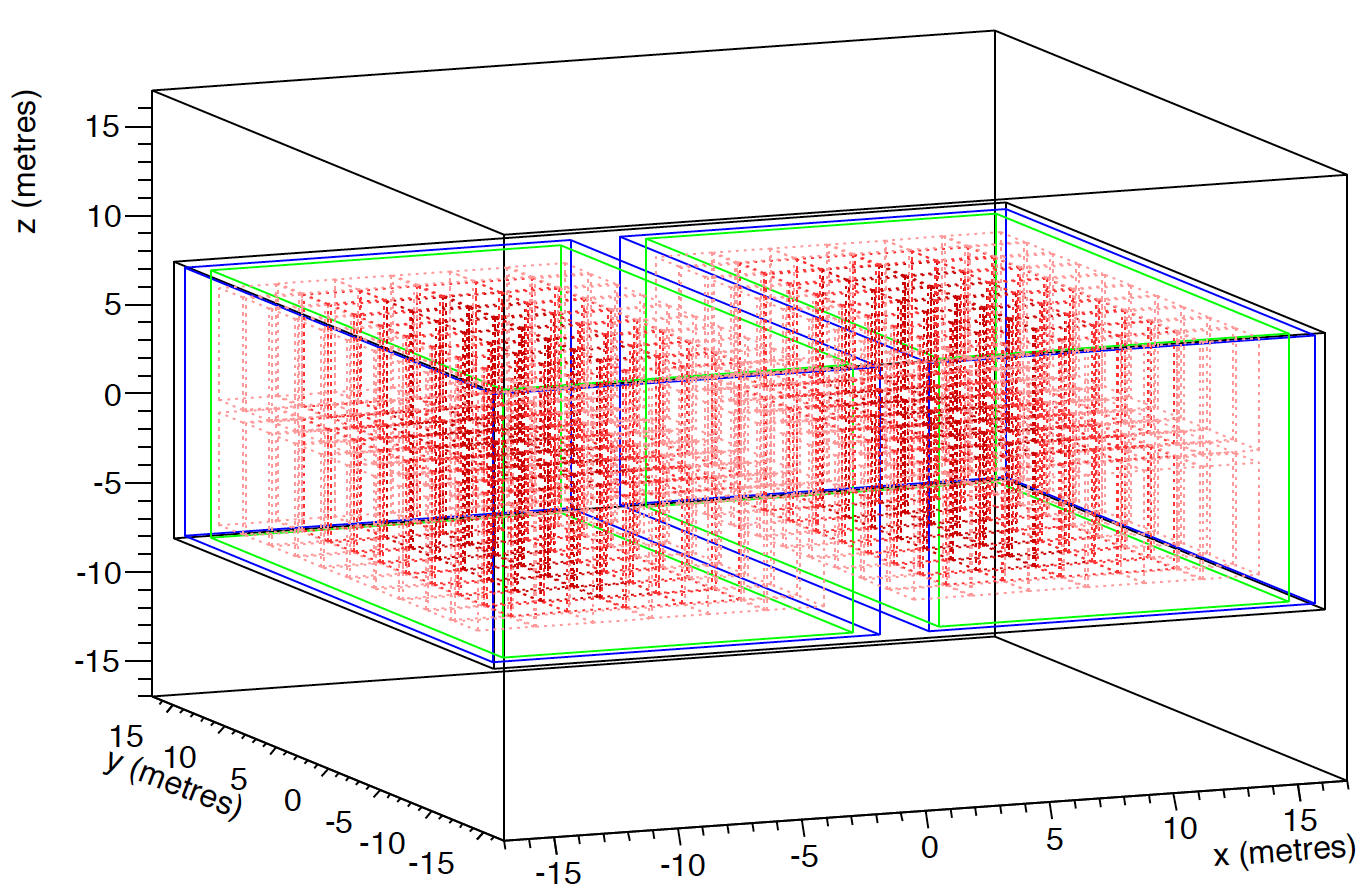
\includegraphics[width=0.8\textwidth]{ComplexGeom}
  \caption[The \emph{complex} detector geometry used in the LBNE surface detector simulations]
          {The \emph{complex} detector geometry used in the LBNE surface detector simulations. The TPC cells are shown in red, and are orientated such that there are 10, 6, and 2 TPCs in the $x$, $y$, $z$ coordinates of each cryostat respectively. The steel walls of the cryostats are green, whilst the outer edges of polyurethane are blue, and the concrete enclosures are black. Figure taken from~\citep{MartinsThesis}.}
  \label{fig:SurfCompGeom}
\end{figure}

Secondly, an accurate surface profile, including the hills surrounding the far detector site was incorporated into the simulations. The proposed location of the LBNE detector was the same as the proposed DUNE detector location, though it was on the surface, and not in the mine. A satellite generated map, centred on SURF, which encompasses an area of 20 $\times$ 20 km$^2$ is used to generate the accurate surface profile. The map is sampled in bins measuring 5 $\times$ 5 m$^2$. To include the effects that the surrounding hills would have on the muon flux, muons are initially sampled 600 m above the surface, and are then stepped through the surface profile, until they reach a box measuring 80 $\times$ 80 $\times$ 36 m$^3$ surrounding the detector. The amount of rock that a muon passes through is calculated, and the energy losses which this will cause are then taken into account before subsequent simulations. By taking the surface profile into account in this way, simulation time can be reduced by not having to simulate the surface profile for every new set of muons. The surface profile is modified so as to have a flat surface measuring 100 $\times$ 100 m$^2$ above the detector location, as it is envisioned that there will be surface facilities around the detector site. The accurate surface profile is shown in Figure~\ref{fig:SurfProf_Col}, where it is presented in the context of producing muons for the DUNE FD location. \\

It should be emphasised that all work presented here has been done using Monte Carlo truth, and so no reconstruction has performed. It also means that at all times only Monte Carlo truth information is used. Therefore, any positions or trajectories which are referred to are those which are recorded by GEANT4~\citep{GEANT4}. This information saved by GEANT4 is ``smeared'' before analysis is performed, in attempt to take into account of some of the detector effects which were not simulated. This smearing is particle type and energy dependant, and is performed on the particles position, trajectory, and energy~\citep{MartinsThesis, LBNE7806}. \\

%%%% Signal / Background events
\subsection{Classifying signal and background events}
Before the simulations can be described in detail, it is necessary to outline what separates a signal event from a background event. In the LBNE and DUNE FD, a $\nu_{e}$ appearance signal event would occur when a $\nu_{e}$ undergoes inelastic scattering with either an electron or nucleon. This interaction will produce an electron, which will in turn produce an EM shower. It is this EM shower which will be identified as a neutrino appearance signal. The electron track which is produced in these interactions will not necessarily be isolated, and may be accompanied by hadronic debris. \\

Cosmic ray particles are able to produce signals which mimic this appearance signal. These signal mimicking events can come from a large variety of sources, including, but not limited to, knock-on electrons from muons, bremsstrahlung photons, meson decays to photons, and EM showers which originate outside of the active volume of the detector but then enter it. A background event is then defined as the initial photon in an EM shower. The first generation photon is used as this will contain the total energy of the shower, and removes the need to record every particle produced in the shower. The final position (point of pair production) of the photon is used in all calculations where the position is required, as the photon will not be observed in the actual detector, only the electrons and positrons it produces. Background showers which start with an electron from Compton scattering are not counted, as pair production is the major source of EM showers at the energies considered here. \\

\subsection{Description of cuts used} \label{sec:SurfCutList}
As noted above, the event rate due to cosmic backgrounds will be much larger than the neutrino event rate, and so a series of cuts, designed to remove cosmic background whilst preserving signal events, have to be developed. This section will briefly outline the cuts which were developed to achieve this. A more rigorous definition of the cuts can be found in~\citep{MartinsThesis}. \\

The simplest cut considers the energy of the electromagnetic (EM) cascade which is induced. As is the case for DUNE, the LBNE beamline was a broadband neutrino beam, where neutrino analyses would have been concentrated within the 0.25 - 5.0 GeV energy range. This means that any EM cascade which deposited more than 5 GeV of energy, or less than 0.25 GeV of energy into the detector would not be considered as a signal event. \\

As charged particles within the detector will produce tracks, it is possible to calculate the minimum separation between these charged tracks and the point at which a photon pair produces. This Point of Closest Approach (PoCA), is calculated by extrapolating the trajectory of the photon backwards from the location at which it pair produces, towards the charged particle tracks. The charged particle tracks are also extrapolated backwards, and so the smallest separations may be outside of the active volume of the detector. A photon is identified as being due to the charged particle track if the PoCA is below a certain threshold. Should a photon be due to a charged particle track, then it is identified as being a background event. Thresholds of 30 cm and 10 cm are used when considering the initial charged muon, and all charged particles respectively. The latter threshold is smaller to avoid removing signal events, and also has a lower limit of 2 cm, meaning that any photons which have PoCAs with respect to any charged particle of less than 2 cm are not identified as background events. This is because it is possible that charged hadrons are produced at the neutrino interaction vertex, and so the electron produced would have a charged particle very close to it, meaning that were this lower limit not in place, this electron would fail the all charged PoCA cut. \\ 

It has been found that the angle of a neutrino event with respect to the neutrino beam is highly correlated to the energy of the neutrino~\citep{barker2012muon}. This means that it is possible to use the angle of a shower with respect to the beam, to distinguish between signal and backgrounds events. The effectiveness of this constraint is highly energy dependant, as any high energy photons which are not tightly correlated to the beam axis will be identified as backgrounds, though few low energy photons will be~\citep{LBNE6621}. Figure~\ref{fig:SurfPoCACut} shows an example of how the PoCA and angle of a photon with respect to the beam axis are calculated. \\

\begin{figure}
  \centering
  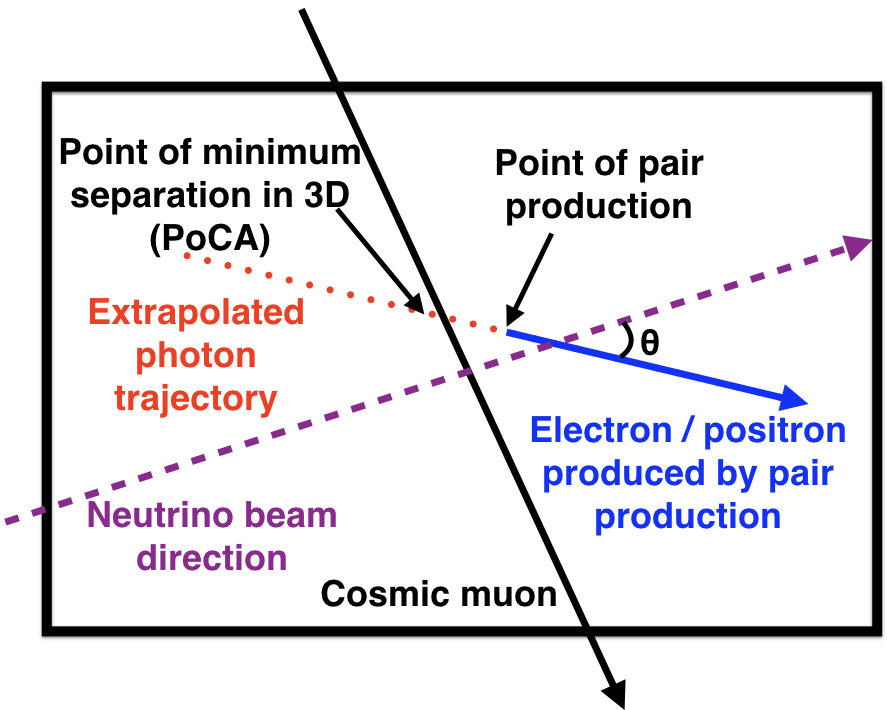
\includegraphics[width=0.6\textwidth]{PoCA_Beam_Cuts}
  \caption[A diagram of the PoCA, and the angle w.r.t the beam calculations in the LBNE surface detector simulations]
          {A diagram of the PoCA, and the angle w.r.t the beam calculations in the LBNE surface detector simulations. A cosmic muon which passes through the detector is shown as a black line, whilst an electron/positron that is produced is shown as a blue line. The minimum distance between the muon and electron/positron is shown (d), as well as the point of closest approach (PoCA) when the electron/positron track is extrapolated backwards. The extrapolated track is shown as a dotted red line. The neutrino beam direction is shown as a dashed green line, and the angle that the electron/positron makes with respect to this is shown ($\theta$). Figure is modified from~\citep{MartinsThesis}.}
  \label{fig:SurfPoCACut}
\end{figure}

It is envisioned that not all of the instrumented LAr will be able to used to identify neutrino events. This is because a fiducial cut will be applied around the detector edges, in order to ensure that the entire track is contained within the active volume of the detector. For the $complex$ detector geometry, this fiducial cut is only applied to the outward facing edges of the active volumes. It is assumed that tracks passing between cells, within a given cryostat, will be able to be stitched together, as is done in LArSoft. \\

Additionally, signal events should be able to be distinguished from background events based on the energy deposition measurements. These will come from identifying the start of an EM shower as coming from either an electron, or a photon, in the case of a signal, and background event, respectively. Studies have shown that the failure rate of this separation tails off at 10\% for showers with energies above 0.5 GeV~\citep{LBNE8458}. Therefore, a flat reduction of $1/10$ is applied to all surviving simulated background events. \\

Finally, it is envisioned that an efficient photon detection system will be used, which uses the scintillation light emitted by excited argon~\citep{PhysRevB.27.5279}. This efficient photon detection system should be able to provide information on individual events, and so identify whether a candidate event occurred within the beam spill. If this is used, then the effective drift time of the detector can be reduced from 1400 $\mu$s to only 10 $\mu$s, a reduction by a factor of 140. This is also applied as a flat reduction to all surviving background events. \\


%%%% Generating particles
\subsection{Generating particles for background studies}
When simulating the cosmogenic background for a detector on the surface it is necessary to simulate the backgrounds due to muons, protons, neutrons and photons. It was found that the background due to cosmic photons was negligible~\citep{MartinsThesis}, and so they are not discussed here. \\

The muons used in the simulations are generated using a Gaisser's parameterisation~\citep{Gaisser}, which has been modified for large zenith angles, and muon decay~\citep{PhysRevD.58.092005}. The differential muon intensity at sea level ($\frac{dI_{\mu}}{dE_{\mu} d\Omega}(E_{\mu}, \theta)$), in units of cm$^{-2}\cdot$s$^{-1}\cdot$sr$^{-1}\cdot$GeV$^{-1}$, is shown in Equation~\ref{eq:Gaisser}.
\begin{equation}
   \begin{aligned}
      \label{eq:Gaisser}
      \frac{dI_{\mu}}{dE_{\mu} d\Omega}(E_{\mu}, \theta) &=
      A \times 0.14\times (E_{\mu} + \Delta)^{-\gamma} \times p_{d} \\
      &\times \left[ \frac{1}{1 + \frac{ 1.1(E_{\mu}+\Delta)cos\theta^{*} }{ 115 GeV } } +
      \frac{0.054}{1 + \frac{1.1(E_{\mu}+\Delta)cos\theta^{*}}{850 GeV}} + R_{c} \right]
   \end{aligned}
\end{equation} 
where $E_{\mu}$ is the muon energy in GeV at the surface, $\theta$ is the muon zenith angle at the surface, $\theta^{*}$ is the muon zenith angle at the height of muon production, $\cos\theta^{*} = \sqrt{1-0.99(1-\cos^{2}\theta)}$, $\Delta$ is the muon energy loss in the atmosphere and is equal to $2.06\times10^{-3} \times \left(\frac{1030}{\cos\theta^{*}} - 120 \right)$, $R_{c}$ is the ratio of prompt muons to pions, and $p_d$ is the probability for a muon to survive in the atmosphere~\citep{PhysRevLett.51.227}. There is also a normalisation constant $A$, and a spectral index $\gamma$, which can both be chosen to fit experimental data. When considering shallow depths, or surface locations, values of $A=1$ and $\gamma=2.7$ are used~\citep{Gaisser}. When considering larger depths, as will be done in Sections~\ref{sec:FDIncorporation} and~\ref{sec:DUNENDK} where MUSUN~\citep{MUSUN, MUSUN2} is used, the typical values are $A=1.84$ and $\gamma=2.77$. These values are taken so as to match the ``depth - vertical muon intensity'' which was measured by the LVD experiment~\citep{PhysRevD.58.092005}. \\

The protons and neutrons used in the simulations are generated using CRY~\citep{CRY,CRY2}, on a plane measuring 50 $\times$ 50 m$^{2}$ in the $xy$ plane. It is not necessary to generate protons and neutrons over a large area as their interaction lengths are much shorter than muons, and so protons and neutrons at large angles which pass through large amounts of rock, will not be a serious concern. The particles are generated at an altitude of 2100 m above sea level. However, the LBNE surface detector would have had an altitude of 1505 m above sea level, and so the particle fluxes generated by CRY have to be corrected to the particle fluxes expected at 1505 m above sea level~\citep{MartinsThesis}. The fluxes generated by CRY are also subject to a further correction, as CRY underestimates the cosmic ray flux by as much as 70\%~\citep{LBNE7517}. This is because CRY only considers protons striking the Earth's atmosphere. As the muon flux is calculated at sea level, this flux also has to be corrected so as to be the flux at 1505 m above sea level~\citep{MartinsThesis}. \\

To reduce simulation time, only particles which will cause most background events are simulated. For example, it is found that 92.7\% of the proton induced background events are due to protons with energies of 10 GeV or more, yet these particles represent only 0.76\% of the total proton flux. This means that by not simulating protons with energies below 10 GeV, the vast majority of background events will be simulated, but this will require less than 1\% of the simulation time. The background events which are not simulated, can be accounted for by correcting the background seen from simulations, by the proportion of background events which were not simulated~\citep{MartinsThesis}. The minimum energies of the simulated muons, protons, and neutrons, along with the percentage of background events which they cause, and the percentage of the particle fluxes above this energy, are shown in Table~\ref{tab:SurfEnPrim}. \\

\begin{table}
  \caption[The minimum energies of simulated particles, when determining the cosmogenic background for the LBNE surface detector]
          {The minimum energies of simulated particles, when determining the cosmogenic background for the LBNE surface detector. The percentage of background events which are caused by particles of these energies, or above, is shown. The percentage of the particle flux above this energy, is also shown. It can be seen that, with appropriate minimum energy constraints, it is possible to avoid simulating over 80\% of the muon flux, 99\% of the proton flux, and 95\% of the neutron flux. Table taken from~\citep{MartinsThesis}.}
  \centering
  \label{tab:SurfEnPrim}
  \begin{tabular}{c c c c}
    \toprule
        {Primary particle} & {Min. energy simulated (GeV)} & {Background (\%)} & {Particle flux (\%)} \\ 
        \midrule
        Muons              & 10                            & 92.3              & 19.6                 \\

        Proton             & 10                            & 92.7              & 0.76                 \\

        Neutrons           & 1                             & 95.6              & 6.5                  \\
    \bottomrule
  \end{tabular}
\end{table}

It can be seen from Table~\ref{tab:SurfEnPrim}, that by only simulating protons above 10 GeV 7.3\% of the background were not simulated, and so the background rate from simulations should be scaled by a factor of 1.0787 $\left(\frac{1}{0.927}\right)$. \\

%%%% Results from simulations.
\subsection{Results from background simulations}
Before the results of the simulations involving the \emph{complex} geometry, and accurate surface profile are discussed, it is useful to briefly summarise the results of the simulations using the \emph{simple} geometry, and flat surface profile. This is shown in Table~\ref{tab:SimpSurfRates}. \\
\begin{table}
  \caption[The normalised background rate per calender year for the \emph{simple} detector geometry, using the flat surface profile]
          {The normalised background rate per calender year for the \emph{simple} detector geometry, separated by particle species, using the flat surface profile. The rates for muons entering the detector, muons missing the detector, proton induced events, and neutron induced events are shown. The annual background for muons entering the detector is only an approximate value, as initial simulations were performed without saving proton hit information, the inclusion of which greatly increases the accuracy of the all charge PoCA cut. Table is taken from~\citep{MartinsThesis}.}
  \centering
  \label{tab:SimpSurfRates}
  \begin{tabular}{l c}
    \toprule
        {Primary particle} & {Annual background rate}  \\ 
        \midrule
        Muons entering     & $\approx$1.18             \\

        Muons missing      & 0.11 $\pm$ 0.02           \\

        Protons            & 2.57 $\pm$ 0.08           \\

        Neutrons           & 1.23 $\pm$ 0.07           \\

        Total              & $\approx$5                \\
    \bottomrule
  \end{tabular}
\end{table}

It can be seen from Table~\ref{tab:SimpSurfRates} that the overall background rate is dominated by hadronic components of the cosmic flux. It is expected that the additional shielding in the \emph{complex} geometry will suppress these components significantly. The annual background induced by cosmic muons has been split into events where the muon enters the detector, and events where it does not enter the detector. This is because when a muon does not enter the detector, the PoCA with respect to the initial muon cannot be calculated. It will also be instructive to observe how the background from each case changes, as the detector geometry is made more accurate. The \emph{complex} geometry, has both a larger surface area and a larger active volume of LAr, therefore it is expected that the muon fluxes will increase. This increase may be quite large for muons which miss the active volume of the detector, as muons may pass through the vertical gaps between TPC volumes and produce secondaries which enter the active volume of the detector. Events like this would, at fist glance at least, appear very similar to a neutrino event, as they will be isolated in the centre of the detector. \\

Only results for the \emph{complex} geometry and accurate surface profile are shown. A separate set of simulations using the \emph{complex} geometry and simple surface profile are shown in~\citep{MartinsThesis}. However, as discussed in~\citep{MartinsThesis}, these background rates were found to be consistent with the background rates for the \emph{complex} geometry and accurate surface profile. \\

Table~\ref{tab:SurfMuComp} shows the background rate for muons which enter the active volume of detector, as sequential cuts are applied, for the \emph{complex} geometry and accurate surface profile. A total of 2 $\times$ 10$^8$ muons with energies greater than 10 GeV are generated, representing 0.1003 years worth of detector live time. The overall number of background mimicking events is seen to increase when using the \emph{complex} detector geometry and the accurate surface profile ($1.32\times10^7$), as opposed to using the \emph{simple} detector geometry and simple surface profile ($1.07\times10^7$)~\citep{MartinsThesis}. It is observed that the expected background rate per calender year for the \emph{complex} detector geometry in the flat ($1.94\pm0.23$), and accurate surface profiles ($2.03\pm0.14$), are consistent~\citep{MartinsThesis}. This means that including the accurate surface profile does not have a significant effect on the background rate. \\

\begin{table}
  \caption[The normalised background rate per calender year, for events where a primary muon enters the active volume of the detector, for the \emph{complex} geometry and accurate surface profile]
          {The normalised background rate per calender year, for events where a primary muon enters the active volume of the detector, for the \emph{complex} geometry and accurate surface profile. A total of 2 $\times$ 10$^8$ muons with energies greater than 10 GeV are generated, representing 0.1003 years worth of detector live time. The background rate is separated into different first generation photon ancestries. The application of the cuts outlined in Section~\ref{sec:SurfCutList} is shown, where $E_\gamma$ is the 0.25 - 5.0 GeV cut, $PoCA_\mu$ is the PoCA w.r.t. the initial muon cut, $\theta_{beam}(E)$ is the energy dependant cut on the angle between the beam and photon trajectory, $PoCA_{all}$ is the PoCA w.r.t. all charged particles cut, $D$ $>$ $30$ is the 30 cm fiducial cut. Following this, two scaling factors of 1/10 and 1/140, representing the e-$\gamma$ separation, and the use of an efficient photon detection system respectively, are applied. The errors quoted are Gaussian, unless the simulated background rate per calender year drops to 0, in which case an upper limit at 90\% confidence level~\citep{PhysRevD.57.3873} is used, with any scaling factors being applied to this limit. No errors are quoted if the error is less than 1\% of the simulated background rate per calender year. Table is taken from~\citep{MartinsThesis}.}
  \label{tab:SurfMuComp}
  \centering
  \scriptsize
  \begin{tabular}{l c c c c c c c c }
    \toprule
        & $E_\gamma$ & $PoCA_\mu$ & $\theta_{beam}(E)$ & $PoCA_{all}$ & $D$ $>$ $30$ cm & $e-\gamma(E)$ & $\gamma$ $detection$ \\
        \midrule
        $Total$          & $1.32\times10^7$ & $(6.38\pm0.09)\times10^4$ & $(2.87\pm0.06)\times10^4$ & $3796\pm229$ & $2854\pm199$ & $285\pm20$   & $2.03\pm0.14$ \\

        $\pi^0\to\gamma$ & $2.24\times10^6$ & $(5.82\pm0.09)\times10^4$ & $(2.62\pm0.06)\times10^4$ & $3339\pm215$ & $2743\pm195$ & $274\pm20$   & $1.96\pm0.14$ \\

        $Ext\to\gamma$   & $4.48\times10^6$ & $5237\pm270$              & $2425\pm183$              & $457\pm80$   & $111\pm39$   & $11.1\pm3.9$ & $0.08\pm0.03$ \\

        $\mu\to\gamma$   & $6.36\times10^6$ & $0-34$                    & $0-15.20$                 & $0-2.01$     & $0-1.51$     & $0-0.15$     & $0-0.001$ \\

        $Other\to\gamma$ & $7.87\times10^4$ & $333\pm68$                & $97\pm37$                 & $0-15.20$    & $0-11.43$    & $0-0.11$     & $0-0.002$ \\
        \bottomrule
  \end{tabular}
\end{table}

The effectiveness of the PoCA cut with respect to the initial muon (2$^{nd}$ column) is obvious, as the annual background event rate is reduced by over 99\%. The rejection rate is observed to be 100\% when considering the $\mu\to\gamma$ photon ancestry (4$^{th}$ row). The rejection rate is also very high in the $Ext\to\gamma$ photon ancestry (3$^{rd}$ row) where it approaches 100\%, this is because when the photons trajectories are extrapolated backwards, they are seen to be very close to the muon track outside the detector. The remaining background is dominated by photons with $\pi^{0}$ parents (2$^{nd}$ row). Around half of the surviving events are removed by the application of the angular cut (3$^{rd}$ column), but more than 80\% of these events are removed by the application of the all charged PoCA cut (4$^{th}$ column). This again shows how powerful the use of the PoCA cut is when rejecting background events. Whilst the fiducial cut (5$^{th}$ column) is seen to be effective at removing the remaining $Ext\to\gamma$ events, this is not the case for the $\pi^0\to\gamma$ events. Therefore, the development of efficient methods of e-$\gamma$ separation (6$^{th}$ column), and the use of an efficient photon detection system (7$^{th}$ column), are critical in reducing the annual background to a rate which would not be prohibitive to observing neutrino interactions. \\

The background rate for the \emph{complex} detector geometry and accurate surface profile, for muons which miss the active volume of the detector, is shown in Table~\ref{tab:SurfMuMissComp}. The same muons used in Table~\ref{tab:SurfMuComp} are used here, meaning that a detector live time of 0.1003 years has been simulated. The overall number of background mimicking events is seen to increase substantially  when using the \emph{complex} detector geometry and the accurate surface profile ($19800\pm500$), as opposed to using the \emph{simple} detector geometry and simple surface profile ($10700\pm300$). This is to be expected, as there is a much larger external surface area, and the vertical gaps produce internal gaps between the TPCs. The expected background rate per calender year for the \emph{complex} detector geometry in the flat ($0.58\pm0.14$), and accurate surface profiles ($0.65\pm0.08$), are consistent, though the total number of background events is less when the accurate surface profile is used ($19800\pm500$ compared to $22100\pm900$)~\citep{MartinsThesis}. \\

\begin{table}
  \caption[The normalised background rate per calender year, for events where a primary muon misses the active volume of the detector, for the \emph{complex} geometry and accurate surface profile]
          {The normalised background rate per calender year, for events where a primary muon misses the active volume of the detector, for the \emph{complex} geometry and accurate surface profile. A total of 2 $\times$ 10$^8$ muons with energies greater than 10 GeV are generated, representing 0.1003 years worth of detector live time. The background rate is separated into different first generation photon ancestries. The application of the cuts outlined in Section~\ref{sec:SurfCutList} is shown. Table is taken from~\citep{MartinsThesis}.}
  \label{tab:SurfMuMissComp}
  \centering
  \scriptsize
  \begin{tabular}{l c c c c c c c }
    \toprule
        & $E_\gamma$ &  $D$ $>$ $30$ cm & $\theta_{beam}(E)$ & $PoCA_{all}$ & $e-\gamma(E)$ & $\gamma$ $detection$ \\
        \midrule
        $Total$          & $19800\pm500$ & $4004\pm235$ & $1551\pm147$ & $914\pm113$ & $91\pm11$      & $0.65\pm0.08$ \\

        $\pi^0\to\gamma$ & $3284\pm213$  & $1108\pm123$ & $526\pm85$   & $166\pm48$  & $16.63\pm4.80$ & $0.12\pm0.03$ \\

        $Ext\to\gamma$   & $16500\pm500$ & $2858\pm199$ & $998\pm118$  & $748\pm102$ & $75\pm10$      & $0.53\pm0.07$ \\

        $Other\to\gamma$ & $28\pm5$      & $28\pm5$     & $28\pm5$     & $0-20$      & $0-2.01$       & $0-0.01$ \\
        \bottomrule
  \end{tabular}
\end{table}

Table~\ref{tab:SurfMuMissComp} shows that muons which miss the active volume of the detector cause much fewer background events than those which strike the active volume of the detector. However, the events which they do cause, are much more likely to survive the application of all cuts. This is due to a combination of both the fiducial cut being less effective, and there being more external photons. Both of these differences are caused by muons which pass through gaps between TPCs, and produce secondaries which are inside the detector walls. These events will produce photons which are not removed by the fiducial cut, and are identified as external photons, as the muon in these events did not produce a track. There will also be more external photons, as the surface area of the detector has substantially increased now that there are two identical cryostats, as opposed to a single block of LAr. \\

Table~\ref{tab:SurfProComp} shows the background rate for protons, as sequential cuts are applied, for the \emph{complex} geometry and accurate surface profile. A total of 1 $\times$ 10$^7$ protons with energies greater than 10 GeV are generated, representing 2.482 years worth of detector live time. As the protons are generated on a plane which measures 50 $\times$ 50 m$^{2}$, and the accurate surface profile was modified to have a flat area above the detector measuring 100 $\times$ 100 m$^{2}$, it is not necessary to propagate protons through the accurate surface profile. As discussed earlier, protons are generated on a plane measuring 50 $\times$ 50 m$^{2}$ as protons will not induce background events at the high inclinations which muons do. The increased overburden causes the overall number of background mimicking events to decrease substantially when using the \emph{complex} detector geometry ($1.55\times10^4$), as opposed to using the \emph{simple} detector geometry (($1.05\pm0.06)\times10^5$). \\

\begin{table}
  \caption[The normalised background rate per calender year, for proton induced events, for the \emph{complex} geometry]
          {The normalised background rate per calender year, for proton induced events, for the \emph{complex} geometry. A total of 1 $\times$ 10$^7$ protons with energies greater than 10 GeV are generated, representing 2.482 years worth of detector live time. The background rate is separated into different first generation photon ancestries. The application of the cuts outlined in Section~\ref{sec:SurfCutList} is shown. Table is taken from~\citep{MartinsThesis}.}
  \label{tab:SurfProComp}
  \centering
  \scriptsize
  \begin{tabular}{l c c c c c c c }
    \toprule
        & $E_\gamma$ &  $D$ $>$ $30$ cm & $\theta_{beam}(E)$ & $PoCA_{all}$ & $e-\gamma(E)$ & $\gamma$ $detection$ \\
        \midrule
        $Total$          & $1.55\times10^4$ & $10559\pm$  & $3475\pm39$ & $319\pm12$ & $31.9\pm1.2$ & $0.23\pm0.01$ \\

        $\pi^0\to\gamma$ & $1.18\times10^4$ & $9277\pm63$  & $3098\pm36$ & $297\pm11$ & $29.7\pm1.1$ & $0.21\pm0.01$ \\

        $Ext\to\gamma$   & $3120\pm37$      & $858\pm19$   & $279\pm11$  & $22\pm3$   & $2.2\pm0.3$  & $0.016\pm0.002$ \\

        $Other\to\gamma$ & $524\pm15$       & $424\pm15$   & $97\pm6$    & $0-1.04$   & $0-0.10$     & $0-0.001$ \\
        \bottomrule
  \end{tabular}
\end{table}

It can be seen from Table~\ref{tab:SurfProComp} that the cut with respect to the beam angle, and the PoCA calculation with respect to all charged particles, are very effective as they remove 67\% and 90\% of all remaining background events respectively. The all charged PoCA cut is effective, since many of the photons produced will be close to the initial proton that was simulated. After all cuts are applied, the annual number of background events is seen to decrease by over a factor of 10 when using the \emph{complex} geometry. This decrease is attributed to the additional shielding which is present in the \emph{complex} geometry, as concrete, insulation and inactive regions of LAr have been added. \\

Table~\ref{tab:SurfNeuComp} shows the background rate for neutrons, as sequential cuts are applied, for the \emph{complex} geometry and accurate surface profile. A total of 1.1 $\times$ 10$^8$ neutrons with energies greater than 1 GeV are generated, representing 0.653 years worth of detector live time. The neutrons are generated on a plane which measures 50 $\times$ 50 m$^{2}$, and so as seen with the protons, it is unnecessary to propagate neutrons through the accurate surface profile. The overall number of background mimicking events is seen to decrease substantially when using the \emph{complex} detector geometry, as opposed to using the \emph{simple} detector geometry. \\

\begin{table}
  \caption[The normalised background rate per calender year, for neutron induced events, for the \emph{complex} geometry]
          {The normalised background rate per calender year, for neutron induced events, for the \emph{complex} geometry. A total of 1.1 $\times$ 10$^8$ neutrons with energies greater than 1 GeV are generated, representing 0.653 years worth of detector live time. The background rate is separated into different first generation photon ancestries. The application of the cuts outlined in Section~\ref{sec:SurfCutList} is shown. Table is taken from~\citep{MartinsThesis}.}
  \label{tab:SurfNeuComp}
  \centering
  \scriptsize
  \begin{tabular}{l c c c c c c c }
    \toprule
        & $E_\gamma$ &  $D$ $>$ $30$ cm & $\theta_{beam}(E)$ & $PoCA_{all}$ & $e-\gamma(E)$ & $\gamma$ $detection$ \\
        \midrule
        $Total$          & $8405\pm113$ & $5697\pm93$ & $1949\pm54$  & $225\pm18$   & $22.5\pm1.8$  & $0.16\pm0.01$ \\

        $\pi^0\to\gamma$ & $6397\pm98$  & $5050\pm87$ & $1744\pm51$  & $194\pm17$   & $19.4\pm1.7$  & $0.14\pm0.01$ \\

        $Ext\to\gamma$   & $1796\pm52$  & $470\pm26$  & $169\pm16$   & $30.1\pm6.7$ & $3.01\pm0.67$ & $0.021\pm0.005$ \\

        $Other\to\gamma$ & $209\pm18$   & $175\pm16$  & $36.2\pm7.4$ & $0-3.68$     & $0-0.37$      & $0-0.003$ \\
        \bottomrule
  \end{tabular}
\end{table}

From Table~\ref{tab:SurfNeuComp} it can be seen that as was the case with the protons, the cut with respect to the beam angle, and the PoCA calculation with respect to all charged particles, are very effective. Upon the application of all cuts, the annual expected background from neutrons in the \emph{complex} geometry is seen to decrease by almost an order of magnitude. Whilst this is not as dramatic as the reduction seen when considering proton induced backgrounds, it still represents a significant reduction in the background rate. This reduction is again attributed to the extra shielding which is present in the \emph{complex} geometry. \\

\subsection{Summary of simulations for the LBNE surface detector}
Taking the sum of the expected background rates from Tables~\ref{tab:SurfMuComp},~\ref{tab:SurfMuMissComp},~\ref{tab:SurfProComp} and~\ref{tab:SurfNeuComp} gives an expected cosmogenic background after cuts for the \emph{complex} detector geometry, and accurate surface profile, of 3.07 $\pm$ 0.25 events per year. This compares with an expected background rate of $\approx$5 events per year, for the \emph{simple} detector geometry, and flat surface profile. The reduction in background rate is due to the additional shielding present in the \emph{complex} geometry which reduces the hadronic background component from 3.80$\pm$0.11 to 0.39$\pm$0.01, a decrease of roughly an order of magnitude. However, the larger surface area of the detector is found to cause the number of background events caused by muons which both enter and miss the active volume of the detector to increase. This increase is very substantial when considering muons which miss the active volume of the detector. This is summarised in Table~\ref{tab:FinalSurfRates}. \\

\begin{table}
  \caption[The normalised background rate per calender year for the \emph{simple} detector geometry and flat surface profile, and for the \emph{complex} geometry and accurate surface profile]
          {The normalised background rate per calender year for the \emph{simple} and \emph{complex} detector geometries, separated by particle species, using the flat and accurate surface profiles respectively. The rates for muons entering the detector, muons missing the detector, proton induced events, and neutron induced events are shown. The annual background for muons entering the detector when using the \emph{simple} detector geometry and flat surface profile is only an approximate value, as initial simulations were performed without saving proton hit information. The inclusion of proton hits greatly increases the accuracy of the all charge PoCA cut, however this was only seen in a small sample. Table is taken from~\citep{MartinsThesis}.}
  \centering
  \label{tab:FinalSurfRates}
  \begin{tabular}{l c c}
    \toprule
        {Primary particle} & {\emph{simp.} geom. \& flat surf. prof.} & {\emph{comp.} geom. \& acc. surf. prof.} \\ 
        \midrule
        Muons entering     & $\approx$1.18     & 2.03 $\pm$ 0.24 \\

        Muons missing      & 0.11 $\pm$ 0.02   & 0.65 $\pm$ 0.08 \\

        Protons            & 2.57 $\pm$ 0.08   & 0.23 $\pm$ 0.01 \\

        Neutrons           & 1.23 $\pm$ 0.07   & 0.16 $\pm$ 0.01 \\

        Total              & $\approx$5        & 3.07 $\pm$ 0.25 \\
    \bottomrule
  \end{tabular}
\end{table}

Following the simulation of large samples of muons, protons, and neutrons, the expected background for the LBNE surface detector is found when considering a \emph{complex} detector geometry, and an accurate surface profile. This is compared to the expected background rate when using a \emph{simple} detector geometry and flat surface profile~\citep{MartinsThesis}. It is observed that the effect of the \emph{complex} detector geometry is to reduce the overall background rate, primarily due to the additional shielding which it provides. This additional shielding causes the proton and neutron induced backgrounds to decrease substantially, as was shown in Table~\ref{tab:FinalSurfRates}. It is however found that there will be a significant source of backgrounds from muons which do not enter the active volume of the detector. This is due to the presence of vertical gaps between the TPC cells. The effect of incorporating the accurate surface profile is found to be negligible, as the hills only offer minimal amounts of shielding. These simulations provide a relatively accurate estimate of the expected background for the LBNE surface design, although it must be stressed that these studies have been performed using Monte Carlo truth information, and so have not used reconstruction. \\

%********************************** % Third Section  *************************************
\section{MUSUN in LArSoft} \label{sec:FDIncorporation}  %Section - X.3
The primary muons in the following discussions are all generated using MUSIC~\citep{MUSUN, MUSIC, MUSIC2} and MUSUN~\citep{MUSUN, MUSUN2}, and so a brief overview of them is required. MUSIC first propagates muons through a medium, defined by the user, for given initial energies. A range of energies between 10$^2$ GeV and 10$^7$ GeV are considered, and their energy distributions are stored at depths of 100 to 15,000 m w.e. Energy losses due to four processes are considered; ionisation, bremsstrahlung, electron-positron pair production and muon-nucleus inelastic scattering. The output of MUSIC, along with the surface muon spectrum parameterisation and the surface profile, is then used by MUSUN to generate a muon energy spectrum and angular distribution, for a given detector location. \\

The location of the DUNE far detector, near the Ross shaft at SURF, has global coordinates of 44$^{\circ}$20$'$45.21$''$ North, 103$^{\circ}$45$'$16.13$''$ West. The rock composition is assumed to be, $< Z >$ = 12.09 and $< A >$ = 24.17. The density is assumed to be 2.70 g$\cdot$cm$^{-3}$~\citep{Mei:2009py}, though some measurements suggest that it may be closer to 2.80-2.90~g$\cdot$cm$^{-3}$~\citep{Gray:2010nc, Heise:2014gta}. The vertical flux calculated by MUSIC/MUSUN of 5.18 $\times$ 10$^{-9}$ cm$^{-2}\cdot$s$^{-1}\cdot$sr$^{-1}$, is well matched to the flux measured by the active veto system of the Davis' experiment, which was (5.38 $\pm$ 0.07) $\times$ 10$^{-9}$ cm$^{-2}\cdot$s$^{-1}\cdot$sr$^{-1}$~\citep{PhysRevD.27.1444}. Given the small differences in these values, and another measurement by the Majorana demonstrator~\citep{Abgrall:2016cfi}, the systematic uncertainty in calculating the muon flux is estimated to be 20\%~\citep{NDKTFNote}. \\

The surface profile around the proposed detector location is shown in Figure~\ref{fig:SurfProf_Col}, where the proposed location is in the centre of the map. Each quadrant on the map has been divided into 4 angles of 22$^{\circ}$ to help guide the eye when comparing it to Figure~\ref{fig:SurfProf_Azi}, where the distribution of azimuth angles is plotted. The vertical lines in Figure~\ref{fig:SurfProf_Azi} show the division of the quadrants when the angle is calculated from East to the North. When moving from East to North it is possible to discern how the peaks and troughs on the surface profile, correspond to troughs and peaks in the distribution of azimuthal angle. \\

\begin{figure}
  \centering
  \begin{subfigure}{0.56\textwidth}
    \centering
    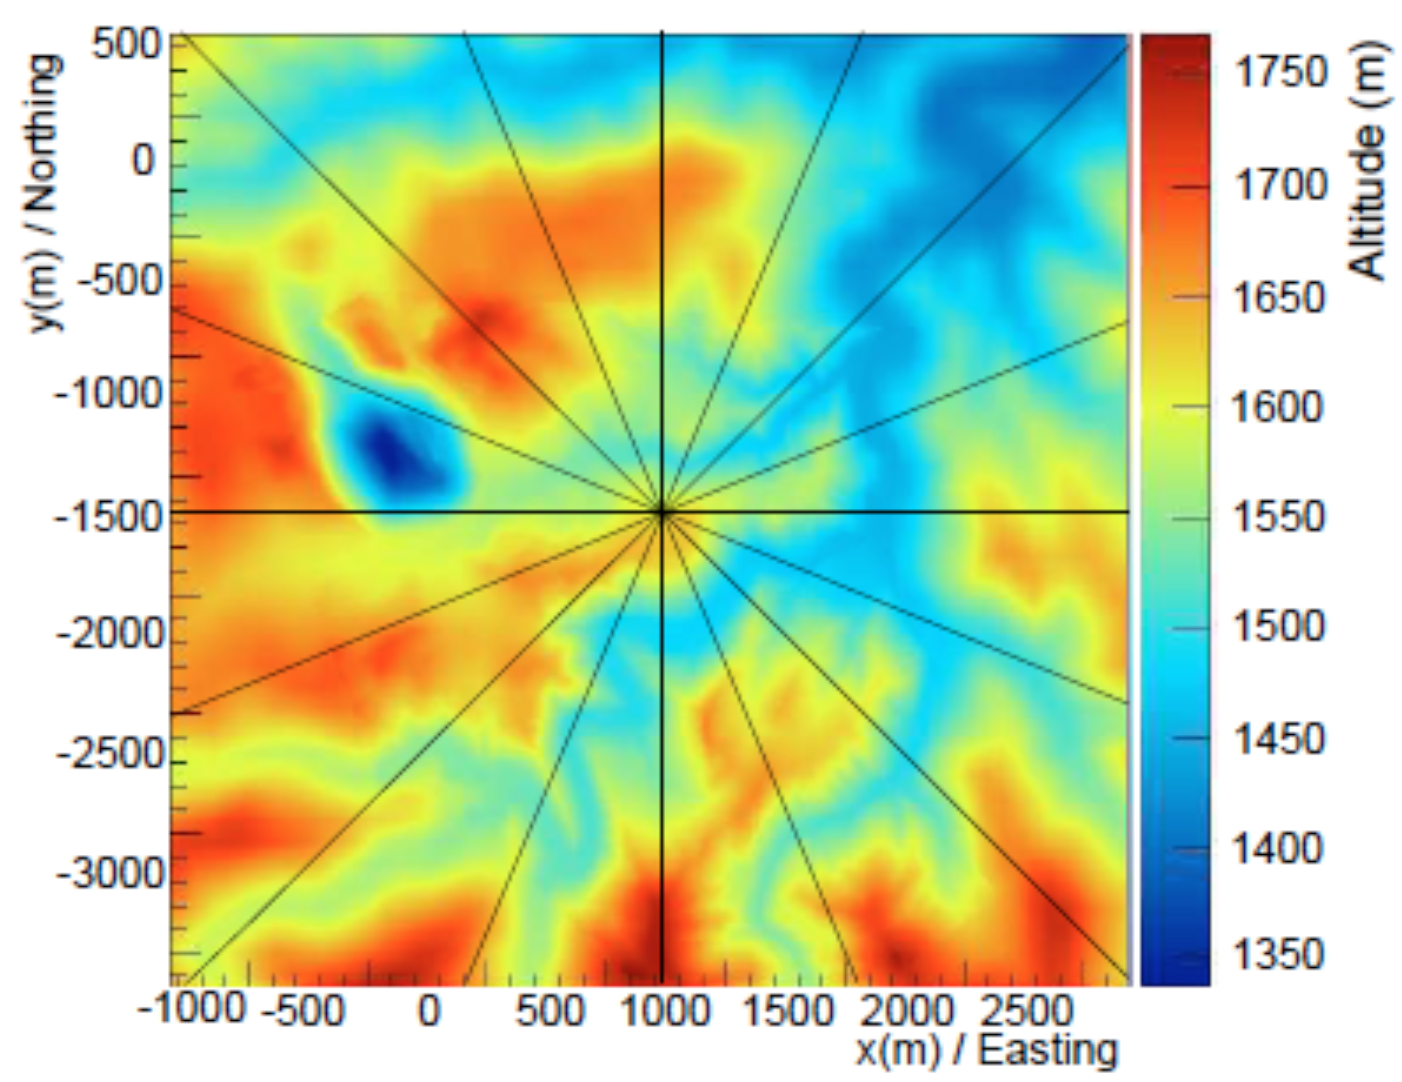
\includegraphics[width=\textwidth]{dune-surface-map}
    \caption{The surface profile of the DUNE far detector site at SURF~\citep{LBNE3144}.}
    \label{fig:SurfProf_Col}
  \end{subfigure}%
  \hspace{0.03\textwidth}%
  \begin{subfigure}{0.4\textwidth}
    \centering
    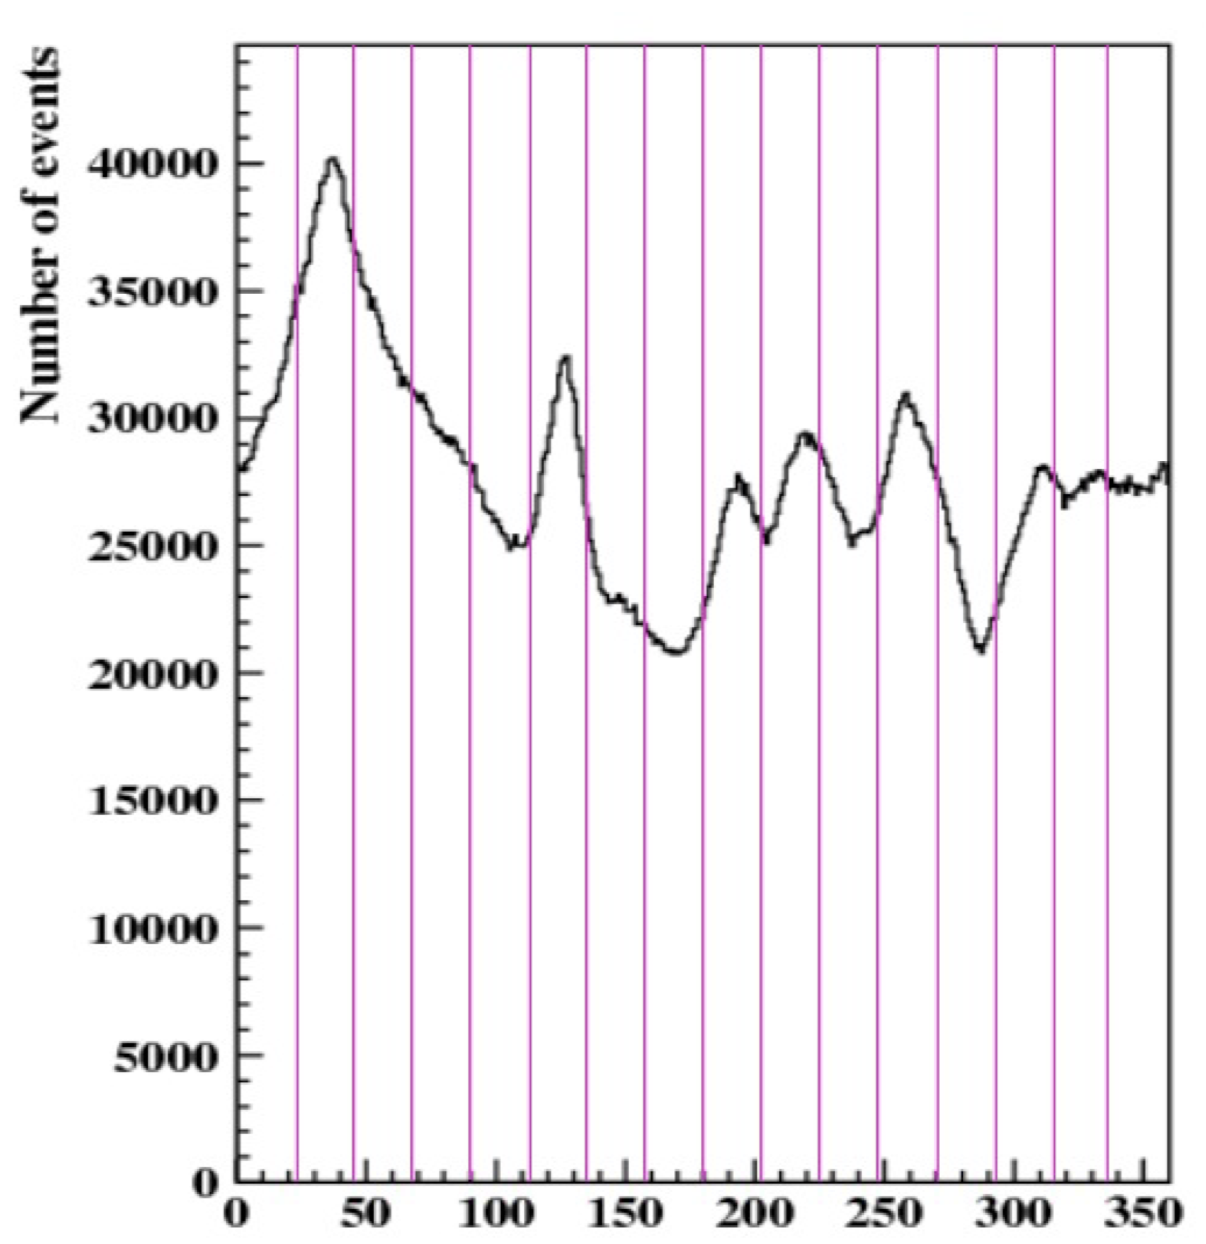
\includegraphics[width=\textwidth]{phi-map}
    \caption{The distribution of azimuthal angles of muons at the DUNE far detector site at SURF~\citep{MartinsThesis}.}
    \label{fig:SurfProf_Azi}
  \end{subfigure}%
  \caption[The correlation between the surface profile, and the distribution of azimuthal angles at the DUNE far detector site]
          {The correlation between the surface profile, and the distribution of azimuthal angles at the DUNE far detector site. The quadrants have been divided into four angles of equal size. The azimuthal angle, calculated as the angle from East (pointing to the right in Fig.~\ref{fig:SurfProf_Col}), and increasing counterclockwise, is seen to follow the contours of the surface profile.}
\end{figure}

Given these parameters, the muon flux at the DUNE far detector location, when assuming a spherical detector geometry, and without simulating a detector cavern, is given in Table~\ref{tab:MUSUNflux}. \\
\begin{table}
  \caption[Muon flux parameters as calculated with MUSIC/MUSUN.]
          {Muon flux parameters as calculated with MUSIC/MUSUN.}
  \centering
  \label{tab:MUSUNflux}
  \begin{tabular}{c c c c}
    \toprule
        {Total flux (cm$^{-2}\cdot$s$^{-1}$)} & {Mean E$_{\mu}$ (GeV)} & {Mean slant depth (m w.e)} & {Mean $\theta$ ($^{\circ}$)} \\ 
        \midrule
        5.66 $\times$ 10$^{-9}$           & 283                    & 4532                       & 26                           \\
    \bottomrule
  \end{tabular}
\end{table}

The muons simulated for DUNE are sampled on the surface of a box surrounding the detector hall, which also encompasses 7 m of rock above the cavern, and 5 m of rock on all other sides. This is to ensure that the simulated muons pass through a sufficient amount of rock to induce cascades, both above and around the detector hall. The secondaries produced in these cascades which enter the detector, in the absence of the initial muon, are of particular interest, as some of them could be mistaken for nucleon decay events. The study of these nucleon decay mimicking events is discussed in Section~\ref{sec:DUNENDK}. The size of the box which the muons are sampled from is 74.43 $\times$ 29.54 $\times$ 30.18 m$^3$, compared to the simulated cryostat which has dimensions, 61.62 $\times$ 14.94 $\times$ 13.58 m$^3$. The dimensions are given as length $\times$ width $\times$ height, using the LArSoft coordinate system which was defined at the start of Section~\ref{sec:LArSoft}. The muons are sampled according to their energy spectrum, for a given zenith and azimuthal angle, using the angular distribution obtained with MUSUN. \\

MUSUN has been incorporated into the DUNE software framework, as it had previously been maintained in FORTRAN as an external package. Before simulations in LArSoft were performed, it was ensured that the muon distributions produced by the ported LArSoft code were identical to the original distributions produced by the FORTRAN code. The distributions produced by the DUNE software framework are shown in Figure~\ref{fig:MUSUNIncorp}, and are consistent with the distributions made for the LBNE collaboration~\citep{MUSUNLBNE}. Figure~\ref{fig:10ktPos} shows the initial positions of 10,000 muons around the simulated DUNE 10 kt module, as generated by LArSoft. The initial positions of the muons are shown as blue points, whilst the cryostat is a single black box, and each TPC is a red box. \\

\begin{figure}
  \centering
  \begin{subfigure}{0.45\textwidth}
    \centering
    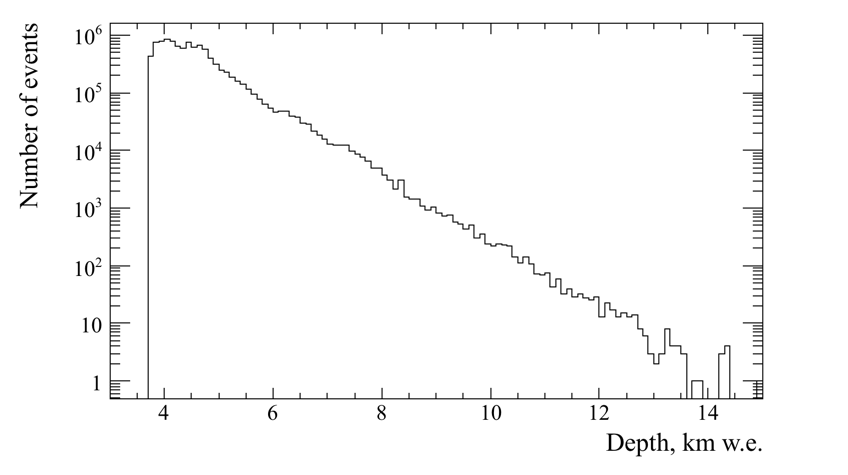
\includegraphics[width=\textwidth]{DepthCan}
    \caption{The number of muons with given slant depths.}
  \end{subfigure}
  \hspace{0.08\textwidth}
  \begin{subfigure}{0.45\textwidth}
    \centering
    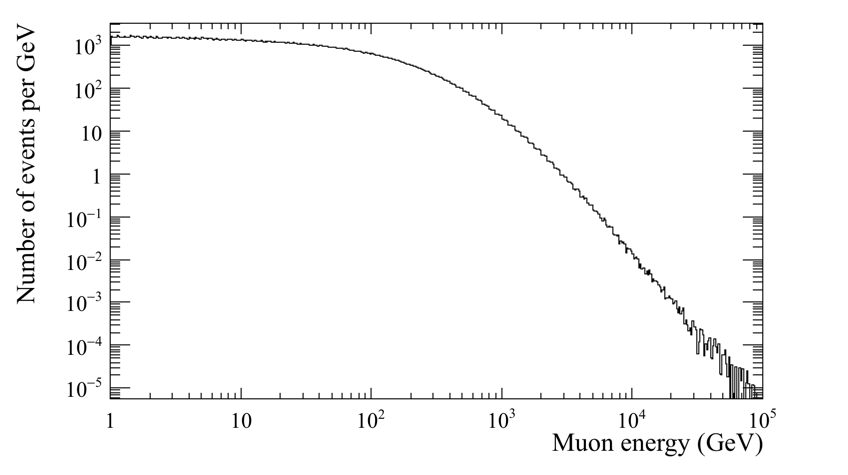
\includegraphics[width=\textwidth]{EnergyPerGeVCan}
    \caption{The initial energy spectrum of simulated muons.}
  \end{subfigure}
  % ========
  \begin{subfigure}{0.45\textwidth}
    \centering
    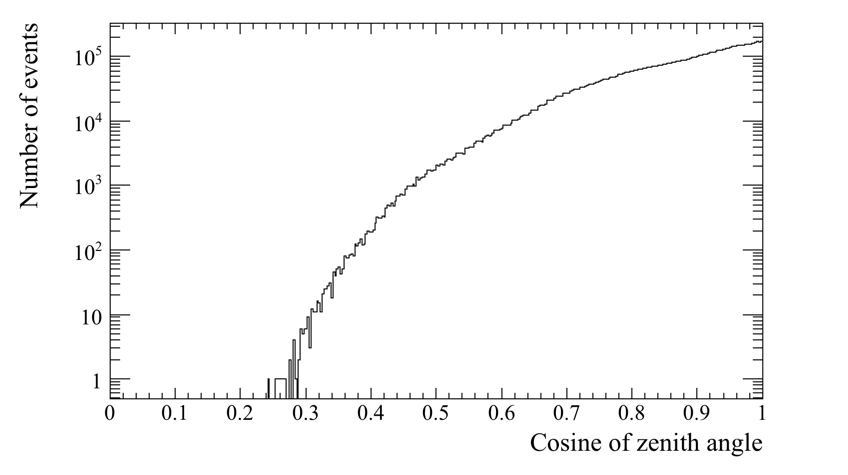
\includegraphics[width=\textwidth]{ZenithCan}
    \caption{The number of muons with given zenith angles.}
  \end{subfigure}
  \hspace{0.08\textwidth}
  \begin{subfigure}{0.45\textwidth}
    \centering
    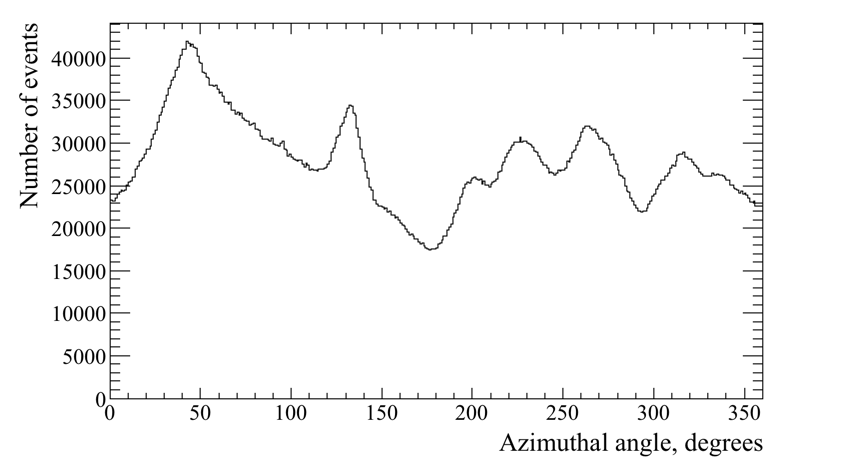
\includegraphics[width=\textwidth]{AzimuthCan}
    \caption{The number of muons with given azimuthal angles.}
  \end{subfigure}
  % ========
  \begin{subfigure}{0.45\textwidth}
    \centering
    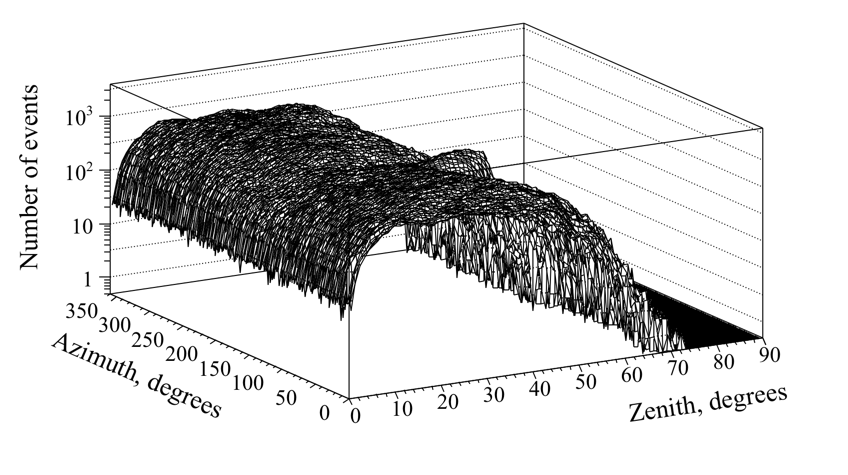
\includegraphics[width=\textwidth]{AziZenCan}
    \caption{The distribution of zenith and azimuthal angles.}
  \end{subfigure}
  \hspace{0.08\textwidth}
  \begin{subfigure}{0.45\textwidth}
    \centering
    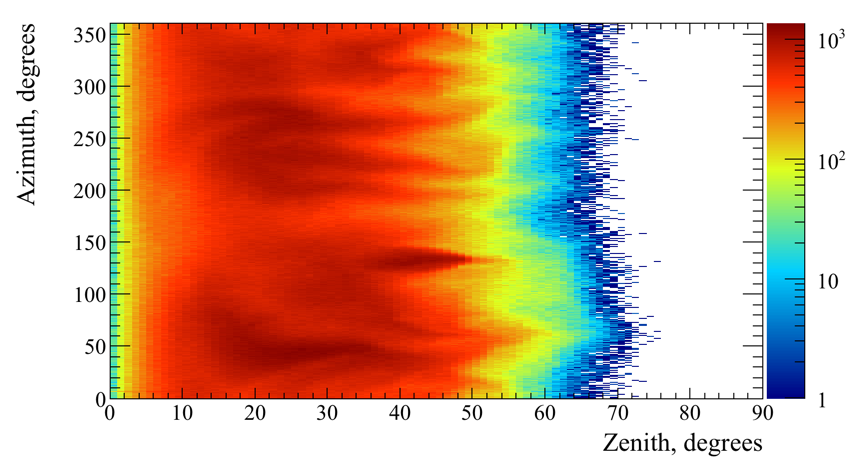
\includegraphics[width=\textwidth]{AziZenColzCan}
    \caption{The distribution of zenith and azimuthal angles, shown with a colour $z$ scale.}
  \end{subfigure}
  \caption[The distributions of muon parameters for a sample of 10$^7$ muons generated by MUSUN in LArSoft]
          {The distributions of muon parameters for a sample of 10$^7$ muons generated by MUSUN in LArSoft. Top left: the slant depths of the simulated muons. Top Right: the energies of the simulated muons. Middle left: the zenith angles of simulated muons. Middle right: the azimuthal angles of simulated muons. Bottom left: the number of muons as a function of zenith and azimuthal angles. Bottom right: the number of muons as a function of zenith and azimuthal angles, as a coloured map.}
  \label{fig:MUSUNIncorp}
\end{figure}

\begin{figure}
  \centering
  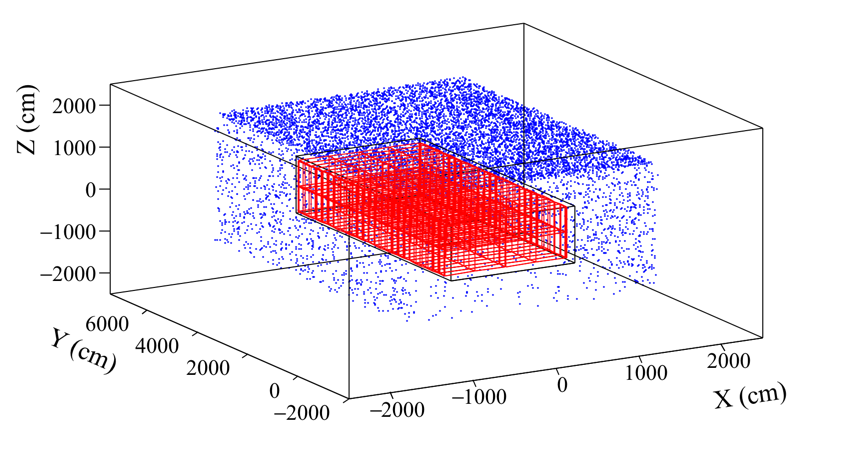
\includegraphics[width=\textwidth]{MuonPosCan}
  \caption[The initial positions of 10$^4$ muons generated by MUSUN around a DUNE 10 kt module]
          {The initial positions of 10$^4$ muons generated by MUSUN around a DUNE 10 kt module. The initial positions of the muons are shown as blue points, whilst the cryostat is a single black box and each TPC is a single red box.}
  \label{fig:10ktPos}
\end{figure}

It is found that the muon rate through the box upon which the muons are sampled is 0.1579 Hz. This rate is later used to normalise the background event rate in Section~\ref{sec:DUNENDK}. Roughly a third of the muons which are generated, pass through the active volume, to give a muon rate through the active volume of 0.053 Hz. \\ 

The simulated far detector is contained in an excavated detector hall surrounded by rock. The cryostat is made of concrete, supported by a stainless steel structure. The inside of the cryostat is filled with LAr, which has a total mass of 17.1 kt. Contained within the cryostat is an active volume of LAr measuring 14.5 $\times$ 12 $\times$ 58 m$^{3}$, made up of 200 TPCs, to give a total mass of active LAr of 14.1 kt. This figure includes gaps between TPCs, when these are removed, the active mass becomes 13.9 kt of LAr. In Section~\ref{sec:DUNENDK} a fiducial cut of 2 cm is used, this causes the fiducial mass to be reduced to 13.8 kt. When performing full energy reconstruction of signal events, this fiducial may have to be increased to ensure that events are fully contained. \\

%********************************** % Fifth Section  *************************************
\section{Nucleon decay channels in DUNE} \label{sec:DUNENDK} %Section - X.5
When searching for rare processes, where an experiment is unlikely to see more than a few signal events, an exhaustive study of the potential backgrounds is required. This is so that if a signal is observed, it could provide overwhelming evidence for the process. The search for nucleon decay in DUNE is one such process, and so an extensive study of the background to nucleon decay is required. As discussed in Section~\ref{sec:BkNDK}, cosmogenic muons cause backgrounds to nucleon decay events, as some of the secondary particles produced by their interactions are able to mimic the nucleon decay signatures. For this reason it is necessary to simulate this background, and to develop a series of cuts which can be applied to the energy depositions which they produce, to establish that they are not due to nucleon decays. When doing this, it is important to use a simulated cosmogenic flux that is as accurate as possible to the one which will be observed by the DUNE far detector. For this reason MUSUN was incorporated into LArSoft, as the muons that it generates correspond to the realistic surface profile, as described in Section~\ref{sec:FDIncorporation}. \\

The DUNE experiment will run for more than 20 years, and so the required statistics for background studies should be even higher than this, so as to ensure the significance of the results. Therefore, a sample of 2 $\times$ 10$^{9}$ muons has been generated. Given that the muon flux through the simulated box is 0.1579 Hz, this sample corresponds to 401.6 years of detector live time for a single DUNE FD module. This sample is thus equivalent to 100.4 years of detector live time for the full DUNE design consisting of four FD modules. \\

Producing samples of this size requires significant computer power, both in terms of running time, and storage space. As a result of this, many of the simulated events are discarded before being saved to disk. This is done through the application of a filter after GEANT4~\citep{GEANT4}, where events satisfying one of the following cuts are discarded;
\begin{itemize}
\item Contains a muon track of more than 1 m.
\item There are no energy depositions in the entire detector volume.
\end{itemize}
This way, events which could mimic nucleon decay signals are not removed from the analyses performed on the large muon sample. In applying these filters it has been assumed that a muon track of more than a metre would definitely be reconstructed. It is also assumed that any signatures observed within one drift window of such a track would not be studied in a nucleon decay search, as there would be doubt as to the authenticity of the signal. Given that the total rate of muons through the active volume is 0.053 Hz, and that the drift time is a few ms, ignoring all times where any track from a cosmogenic muon is present results in less than 0.1\% dead time. The dead time associated with ignoring events with muon tracks of more than 1 m is clearly less than this. This fraction of dead time is assumed to be acceptable. Filtering out events where there are no energy depositions in the detector is clearly acceptable, as there are no energy depositions which could mimic a nucleon decay signature. \\

After applying this series of cuts, 98.12\% of the initial muon sample are removed, meaning that the initial sample of 2 $\times$ 10$^9$ muons is reduced to around 4 $\times$ 10$^{7}$ muons. This is a much more reasonable sample size to store on disk, and to perform analyses on. It is upon this reduced sample of muons that the cosmogenic background analyses are performed. As discussed in Section~\ref{sec:DUNE_NDK}, the proton decay channel of $p \rightarrow K^{+} + \overline{\nu_{e}}$ is referred to as the 'Golden Channel' in LAr, this analysis is discussed in~\citep{NDKTFNote}. The related decay of a neutron in the decay $n \rightarrow K^{+} + e^{-}$ is discussed here. The theoretical motivation for this channel was briefly discussed in Section~\ref{sec:Theory_NDK}. \\

%********************************** % Fifth.First Section  *************************************
\subsection{Cosmogenic background to the $n \rightarrow K^{+} + e^{-}$ decay channel} \label{sec:NDKCosmBk}
As was shown in Table~\ref{tab:NDKLim}, the predicted sensitivity that DUNE will have to this channel is much better than that of Super-K. As a result, it is an interesting decay mode to study. As discussed in Section~\ref{sec:BkNDK}, the cosmogenic background to nucleon decay is predominantly caused by neutral particles, such as a $K^0$, entering the detector volume, and interacting relatively far from the detector edges. This is particularly true for the 'Golden Channel,' as shown in Figure~\ref{fig:K0LongBackground}, but it also holds for other channels. Events like this are the main cause for concern when eliminating all cosmogenic backgrounds. As mentioned in Section~\ref{sec:BkNDK}, it is difficult to separate a $K^+$ from a $K^-$ in a LArTPC, and so any charged kaon is considered a background in the analysis which is presented in this thesis. \\

The analysis presented in this thesis has been performed on Monte Carlo truth information, and so does not contain any reconstructed quantities. Studies involving hit and track reconstruction are in progress~\citep{CosmoJanCollabMeeting}, though they will not be discussed here. As Monte Carlo truth information has been used, perfect particle identification (PID) has been assumed. There was also no smearing of the energies, locations, or trajectories of any simulated particles, meaning that it is assumed that all deposited charge will be reconstructed, and that the detector characterisation is perfect. The energy cuts which are applied in Section~\ref{sec:NDKEnCosmBk} do allow for energy smearing to be taken into account though, as they can easily be made wider than the true distributions. The omission of smearing is something which will need to be refined in future analyses, and will be taken into account when the analysis progresses to use reconstructed quantities, as discussed in Section~\ref{sec:NDKImprov}. \\ 

As is the case with the 'Golden Channel,' the final state of the decay contains a single charged kaon, and so events which do not contain a kaon track can be immediately discounted. There is also an electron in the final state of the decay, and so this means that events which do not also contain an electron can be discounted. In a nucleon decay event, the kaon and electron produced in the final state will have a common vertex, and so the requirement that the two particles have a common vertex can also be applied. Other constraints that are applied to eliminate background events are; a cut on external muon track length in the active LAr, a cut on depositions near the detector edges, and criteria about the distribution of deposited energy. The criteria about the distribution of deposited energy are found by considering a sample of simulated neutron decay events, and are discussed in Section~\ref{sec:NDKEnCosmBk}. These cuts, applied sequentially, are outlined below:
\begin{itemize}
\item The event contains energy depositions due to kaons and due to electrons.
\item The event contains at least one kaon track, and at least one electron track/shower.
\item The event contains a single kaon track, and a single electron track/shower.
\item No external muon travels more than 20 cm in the active detector volume.
\item The event has no energy depositions within 2 cm of the detector edges.
  \begin{itemize}
  \item This is changed to a maximum of 10 MeV of energy deposited within 2 cm of the detector edge, for reasons which will be discussed in Section~\ref{sec:NDKSig}.
  \end{itemize}
\item The kaon and electron share a common vertex, defined as:
  \begin{itemize}
  \item The kaon and electron tracks being separated by no more than 5 cm.
  \item If the kaon and electron tracks are separated by more than 5 cm, then the point of closest approach between the two extrapolated tracks is less than 2 cm.
  \end{itemize}
\item The energy depositions in the event are within the ranges expected from a nucleon decay event. This is explained in Section~\ref{sec:NDKEnCosmBk}, but the energies considered are summarised below:
  \begin{itemize}
  \item The energy directly deposited by the kaon and its secondaries, excluding its decay products.
  \item The energy deposited by the kaon decay products and any of their secondaries.
  \item The energy directly deposited by the electron and its secondaries.
  \item The energy deposited near the shared kaon and electron vertex that is not associated with the kaon or electron.
  \item The energy deposited in the detector which does not fit any of the above criteria.
  \end{itemize}
\end{itemize}

When performing the analysis it is important to be able to trace the particle ancestry. This is so that energy depositions in the detector can be properly assigned to the relevant particles. For example, a $\mu^{+}$ is often produced when a $K^{+}$ decays at rest, and this muon may travel more than 20 cm. However, the cut on muon track length should not be applied to this muon as it was produced by the decay of the kaon. Similarly, as the kaon interacts in the detector, secondary particles will be produced which will be reconstructed as tracks coming off the main kaon track. The initial kinetic energy of the kaon can only be determined by summing the energy depositions due to these secondary particles, and the energy depositions due to the kaon itself. Correctly calculating the initial kaon kinetic energy is critical when determining if an event is a nucleon decay event. The reason for this is that nucleon decay events have very specific energy spectra, and so being able to correctly assign the ancestry of energy depositions is vitally important. The same is true for the electron energy, which is calculated by tracing the ancestry of the particles produced in the EM shower which it produces back to the electron. \\

As no reconstruction has been performed, the tracks referred to here are different from those in Chapters~\ref{chap:35tonSim} and~\ref{chap:35tonData}. The definition of a track used here, is that the particle in question has energy depositions, on simulated wires, which are directly associated with it. These simulated wires are not the same as the wires which have been considered in Chapter~\ref{chap:35tonSim}, as the simulated signals have not been digitised. This distinction is important, as it allows the energy depositions directly from GEANT4 to be used, whilst also allowing for LArSoft methods concerning whether depositions are within TPC boundaries, to be utilised. \\

The simulated electrons may begin showering immediately, or they may produce a short ``track like'' segment before beginning to shower. To ensure that every electron shower can be identified, electrons are not required to produce a short ``track like'' segment. This means that all electrons are assumed to begin showering immediately, and it is also assumed that all of the energy in the shower can be identified as coming from a single electron. This definition of shower energy is the one that is used when the showering algorithms are developed in LArSoft. It is hoped that when DUNE begins taking data the showering algorithms will be able to achieve this level of energy reconstruction. \\

When calculating the distance between the start of the kaon track, and the start of the electron track/shower, the energy depositions whose locations are closest to the Monte Carlo truth start points of the particles are used. For particles which are produced within the active volume, these locations generally correspond to the Monte Carlo truth start positions, though this is not always the case. For example, if a particle is created in the gap between two TPCs, then there will be no charge collected until it enters the active volume. This will result in the measured start position to be shifted from the true generation point. This shift can prove troublesome when considering decay events, as if the decay occurred in the centre of an APA, then it is likely that the kaon and electron would deposit energy on opposite sides of the APA. This could cause the depositions to be separated by over 5 cm, as this is the width of the APAs. However, if the tracks are propagated backwards, towards their true start point, it should still be possible to determine that they had a common vertex. An example of a simulated decay event where this happens is shown in Figure~\ref{fig:NDK_Sig_KEBigGap}. \\

\begin{figure}
  \centering
  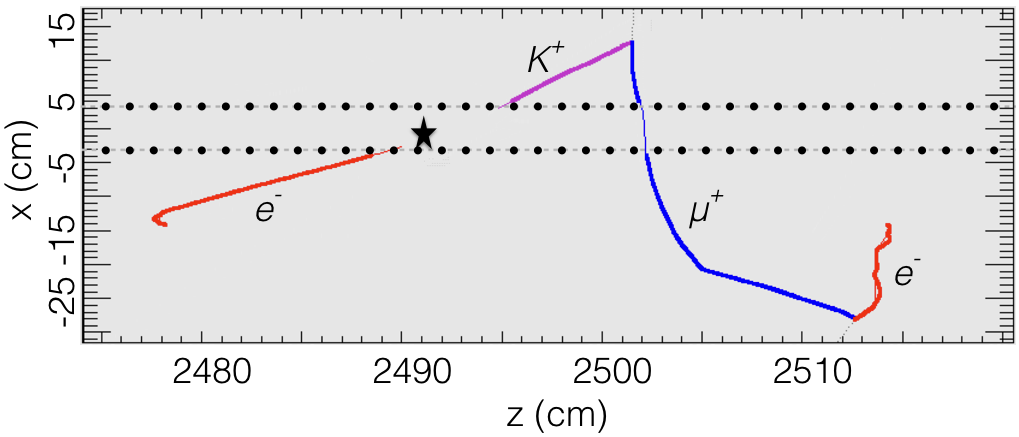
\includegraphics[width=0.8\textwidth]{KaonElecBigGap}
  \caption[A simulated $n \rightarrow K^{+} + e^{-}$ decay which occurred in a gap between TPCs]
          {A simulated $n \rightarrow K^{+} + e^{-}$ decay which occurred in a gap between TPCs. The path of the kaon produced in the decay is shown as a purple line. The path of the muon, produced by the decay of the kaon, is shown as a blue line. The paths which the electrons in the event took are shown as red lines. The electron on the left of the figure is the electron produced in the neutron decay, whilst the one on the right of the figure, is produced by the decay of the muon. The thin coloured lines show track segments which were in uninstrumented parts of the detector, such as gaps between TPCs and APAs. The dotted black lines show the edges of the TPCs, and the black star shows the location at which the decay occurred. The distance between the first kaon energy deposition, and the first electron energy deposition, is found to be 10.7 cm. However, when the kaon and electrons tracks are extrapolated towards the true start position, the point of closest approach (PoCA) between the two tracks is found to be 0.67 cm. This shows that they do in fact have a common vertex, despite the large separation of the start points.} 
  \label{fig:NDK_Sig_KEBigGap}
\end{figure}

In order for a kaon track and an electron shower to be considered to share a common vertex, the separation between the start of the kaon track and the start of the electron shower, must be no more than than 5 cm. A maximum separation of 5 cm is used, as, if the two particles are produced in the centre of a TPC, a gap of 5 cm would require no energy depositions to be collected over approximately 10 collection wires. This is assumed to be unlikely during data taking, and cannot happen in the simulations considered here, as Monte Carlo truth information is used. However, as shown by Figure~\ref{fig:NDK_Sig_KEBigGap}, it is possible for the kaon and electron produced in a signal event to be separated by more than 5 cm. To prevent events such as this being missed, a second criteria is applied to events with large separations. This criteria is that the ``Point of Closest Approach'' (PoCA) between the two particles, found by extrapolating the kaon track and the electron shower forwards and backwards, is less than 2 cm. This is the same PoCA calculation which was made in Section~\ref{sec:SurfCutList}, and it means that events such as the one shown in Figure~\ref{fig:NDK_Sig_KEBigGap} are still identified as signal events. \\

The fiducial cut is only applied to the outer edges of the cryostat, as if it were done with respect to the edge of every TPC in the far detector the loss of volume would be non-negligible. This means that the event shown in Figure~\ref{fig:NDK_Sig_KEBigGap} would not fail the fiducial cut, as the decay occurred over 6 m away from the edge of the detector, but happened to be in a gap between two TPCs. The need for a fiducial cut is two fold, firstly the vast majority of cosmically induced events in the detector will have a charged particle which enters the detector. Performing a fiducial cut will remove all of these events, and will then mean that the only cosmic background events which can mimic a signal event would involve either a significant amount of charge being missed, or a neutral particle entering the detector, and interacting relatively far from the detector walls. Secondly, in order to calculate the kinetic energies of the particles produced in the nucleon decay, and also to perform particle identification, they must be fully contained within the detector. As such, if one of the particles produced in the nucleon decay escapes the detector then it's kinetic energy cannot be determined accurately, and if it is the kaon, or its decay products, then the particle cannot be identified using the method discussed in Section~\ref{sec:PID}. This will also affect any particles which stop in the gaps between TPCs, as the end point will not be reconstructed, though PID may still be possible as the end point can be estimated. A fiducial cut of 2 cm is used, as the loss of active volume which this causes is negligible in the DUNE FD. A 2 cm fiducial cut also ensures that a significant amount of charge would have to be missed for a particle which enters/escapes the detector to be incorrectly identified as being contained within the detector. \\

Once both the ancestry of energy depositions in the simulation, and the initial kinetic energies, have been correctly accounted for and calculated, it is possible to observe the distribution of background events as the cuts outlined above are applied. The energy distribution of background events surviving the application of sequential cuts is shown in Figure~\ref{fig:NDK_CosmoBack_Raw}. The energy distribution of background events per MeV of energy deposited, surviving the application of sequential cuts is shown in Figure~\ref{fig:NDK_CosmoBack_Norm}. This distribution is obtained by dividing the number of events within an energy bin by the bin width. \\

\begin{figure}
  \centering
  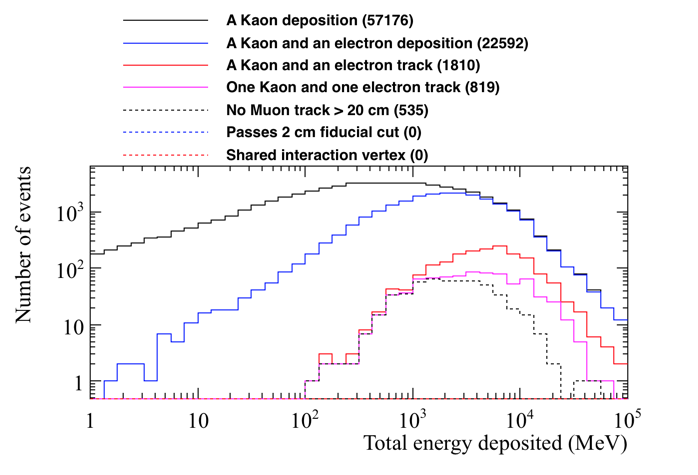
\includegraphics[width=0.8\textwidth]{CosmicBackground_EnergyDepCuts_Raw_2cmCut}
  \caption[The energy distribution of background events surviving the application of sequential cuts.]
          {The energy distribution of background events surviving the application of sequential cuts. The total energy deposited in the detector is plotted on the $x$ axis. A sample of 2 $\times$ 10$^9$ muons, representing 401.6 years of detector for a single FD module is shown.}
  \label{fig:NDK_CosmoBack_Raw}
\end{figure}

\begin{figure}
  \centering
  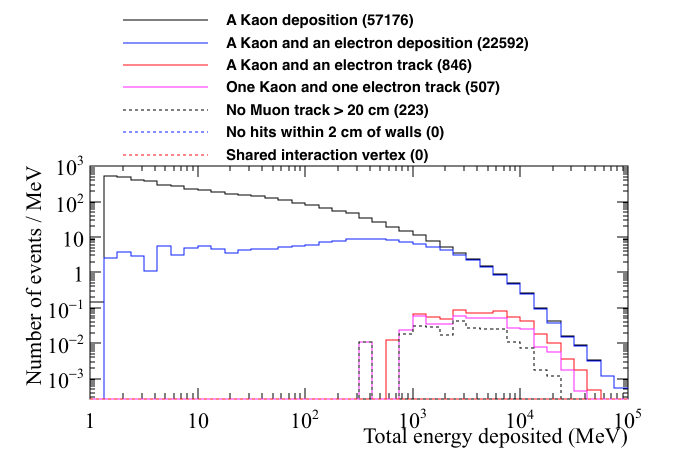
\includegraphics[width=0.8\textwidth]{CosmicBackground_EnergyDepCuts_Norm_2cmCut}
  \caption[The energy distribution of background events per MeV of deposited energy surviving the application of sequential cuts]
          {The energy distribution of background events per MeV of deposited energy surviving the application of sequential cuts. The total energy deposited in the detector is plotted on the $x$ axis. This distribution is obtained by dividing the number of events within an energy bin by the bin width. A sample of 2 $\times$ 10$^9$ muons, representing 401.6 years of detector for a single FD module is shown.}
  \label{fig:NDK_CosmoBack_Norm}
\end{figure}

From Figures~\ref{fig:NDK_CosmoBack_Raw} and~\ref{fig:NDK_CosmoBack_Norm}, it can be seen that there are no background events which could mimic a decay signature, as no events survive the application of all cuts. This corresponds to a limit of the background rate of less than 0.44~events$\cdot$Mt$\cdot$year at the 90\% confidence level, using double sided errors~\citep{PDGReview} and a fiducial mass of 13.8 kt to give an exposure of 5.542~Mt$\cdot$year. \\

It is interesting to observe the effect that relaxing some of the cuts has on the background rate. For example, the cuts after the requirement that there be at least one kaon track and at least one electron shower in the event, could be relaxed. This is shown in Table~\ref{tab:NDK_CosmoBack_EachCut}, where the later cuts have been applied in isolation to observe their effectiveness. \\

\begin{table}
  \caption[The number of events which could mimic a $n \rightarrow K^{+} + e^{-}$ decay, when cuts are applied in isolation]
          {The number of events which could mimic a $n \rightarrow K^{+} + e^{-}$ decay, when cuts are applied in isolation. Cuts are applied after it is required that the event contains at least one kaon track and at least one electron shower. It is found that 1393 events have at least one kaon track and at least one electron shower, this is shown in the top row of the table. The fiducial cut of 2 cm is seen to remove almost all of the events considered.}
  \centering
  \label{tab:NDK_CosmoBack_EachCut}
  \resizebox{\columnwidth}{!}{%
  \begin{tabular}{c c c}
    \toprule
        {Cut that is applied}                                & {Num. events surviving cut} & {\% surviving}\\
        \midrule
        At least one kaon track, and electron shower         & 1393                        & 100        \\

        Only one kaon track, and only one electron shower    & 606                         & 43.5       \\

        No muon track that is longer than 20 cm in length    & 1223                        & 87.8       \\

        No energy depositions within 2 cm of detector edge   & 5                           & 0.359      \\

        The kaon and electron share a common vertex          & 64                          & 4.59       \\
        \bottomrule
  \end{tabular}%
  }
\end{table}

The effectiveness of the fiducial cut is clearly apparent from Table~\ref{tab:NDK_CosmoBack_EachCut}, as it removes all but 5 of the 1393 events where there is both a kaon track and an electron shower. The requirement that the kaon track and electron shower share a common vertex is also seen to be very effective at removing background events, as only 64 of the 1393 meet this condition. When the cuts are no longer applied in isolation, but are instead applied in a different order to that used when producing Figures~\ref{fig:NDK_CosmoBack_Raw} and~\ref{fig:NDK_CosmoBack_Norm}, it is found that in only 15 of the 606 events that have a single kaon track and a single electron shower, would the kaon and electron be considered to have a common vertex. When the additional constraint of there not being an external muon with a track length of more than 20 cm present in the detector is applied, 10 of the remaining 15 events background events would still not be removed. This shows that the only way to remove all of the background events is to apply all of the cuts which have been developed, including the fiducial cut. \\

%********************************** % Fifth.Second Section  *************************************
\subsection{Signal events in the $n \rightarrow K^{+} + e^{-}$ decay channel} \label{sec:NDKSig}
It is important to confirm that the cuts developed to reject cosmic backgrounds do not adversely affect the identification of nucleon decay events. For this reason, a sample of 10,000 neutron decay events in the DUNE far detector were generated using GENIE version 2.12.2~\citep{GENIE}, and the so-called \emph{hA} model of intranuclear effects. Studies have been done comparing the different models for intranuclear effects in GENIE~\citep{FDTFMarch2017}, and future nucleon decay studies may be modified to use the so-called \emph{hN2015} model. The \emph{hA} model does not simulate any $K^+$ charge exchange or absorption, whereas the \emph{hN2015} model does. As a result, the \emph{hN2015} model predicts that more protons and neutrons will be emitted from the nucleus in final state interactions~\citep{FDTFMarch2017}. Neutron decays are generated at random positions within the detector volume, and so it is possible that the decay occurs in the gaps between TPC volumes, as shown in Figure~\ref{fig:NDK_Sig_KEBigGap}, or near the edge of the detector, as is shown in Figure~\ref{fig:NDK_Sig_KENearEdge}. However, many of the neutron decay events are fully contained within a single TPC, as shown by Figure~\ref{fig:NDK_Sig_Cont}. \\

\begin{figure}
  \centering
  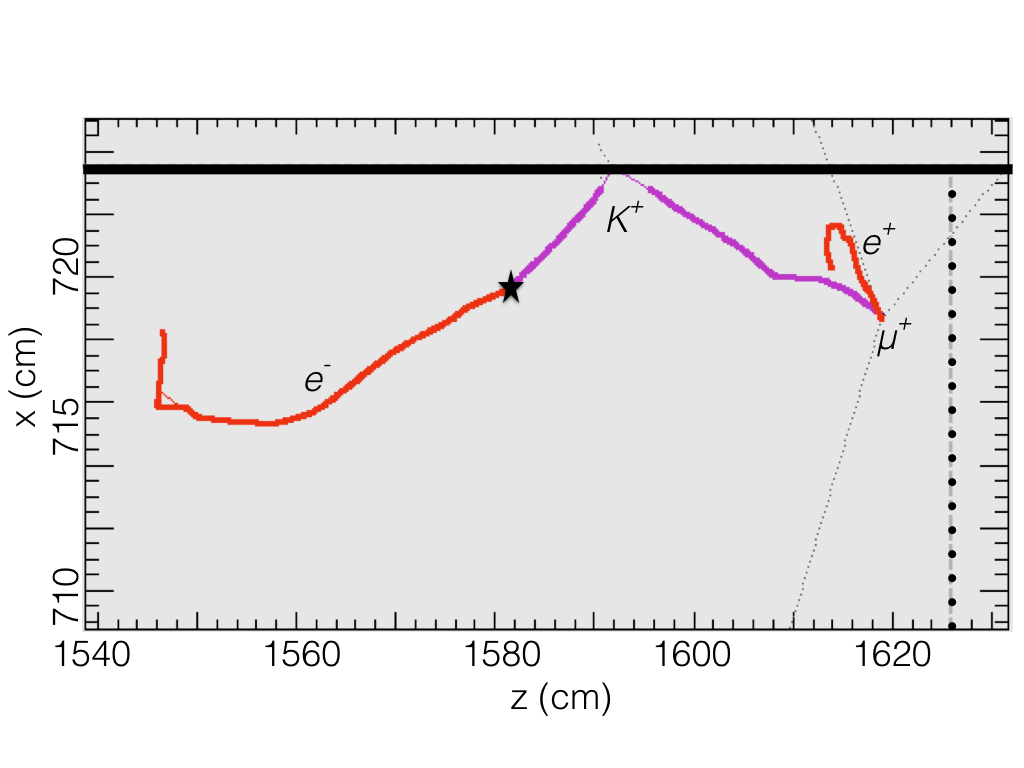
\includegraphics[width=0.8\textwidth]{NearEdgeDecay}
  \caption[A simulated $n \rightarrow K^{+} + e^{-}$ decay which occurred near the edge of the detector volume]
          {A simulated $n \rightarrow K^{+} + e^{-}$ decay which occurred near the edge of the detector volume. The path of the kaon produced in the decay is shown as a purple line. The path of the muon, produced by the decay of the kaon, is shown as a blue line, though it is very short and so barely visible. The paths which the electrons in the event took are shown as red lines. The electron on the left of the figure is the electron produced in the neutron decay, whilst the one on the right of the figure, is produced by the decay of the muon. The thin grey lines show spallation neutrons. The thin coloured lines show track segments which were in uninstrumented parts of the detector, such as the edge of the active volume. The solid black line shows the edge of the detector. The dotted black lines show the edges of the TPCs, and the black star shows the location at which the decay occurred. It can be seen that though most of the energy depositions are contained within the detector, the kaon passes very close to the edge of the detector, and so some of its charge is not reconstructed. The proximity of the decay to the detector walls causes there to be a large amount of charge deposited near the edge of the detector.}
  \label{fig:NDK_Sig_KENearEdge}
\end{figure}

\begin{figure}
  \centering
  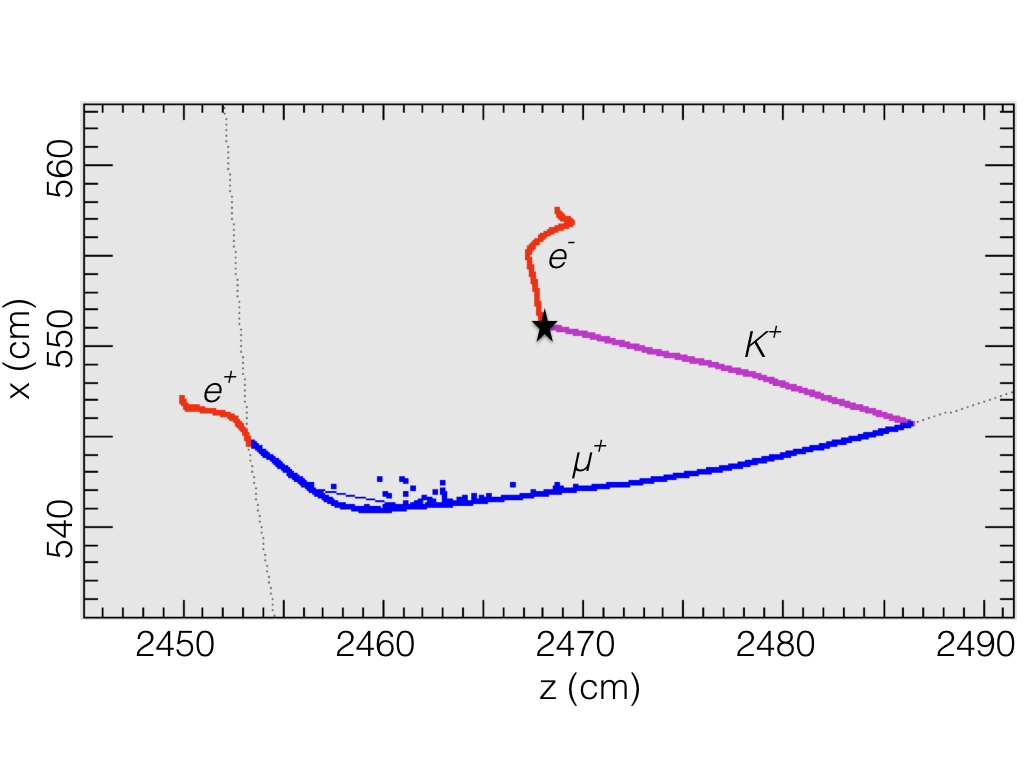
\includegraphics[width=0.8\textwidth]{FullyContained}
  \caption[A simulated $n \rightarrow K^{+} + e^{-}$ decay which is fully contained in a single TPC volume]
          {A simulated $n \rightarrow K^{+} + e^{-}$ decay which is fully contained in a single volume. The path of the kaon produced in the decay is shown as a purple line. The path of the muon, produced by the decay of the kaon, is shown as a blue line. The paths which the electrons in the event took are shown as red lines. The electron at the top of the figure is the electron produced in the neutron decay, whilst the one at the bottom left of the figure, is produced by the decay of the muon. The thin grey lines show spallation neutrons. The black star shows the location at which the decay occurred. It can be seen that all of the deposited charge is contained within a single TPC.}
  \label{fig:NDK_Sig_Cont}
\end{figure}

The analysis performed on the cosmogenic background was primarily designed to reject background events, whilst also attempting to not use cuts which would also affect signal efficiency. Therefore, it is hoped that the loss of signal events will be minimal. When running the analysis on the simulated signal events, the same definitions for tracks, showers, and the ancestry of particles are used, as well as the same cuts that were outlined in Section~\ref{sec:NDKCosmBk}. \\

The energy distribution of the signal events surviving the application of the sequential cuts is shown in Figure~\ref{fig:NDK_Sig_Raw}, this is the equivalent of Figure~\ref{fig:NDK_CosmoBack_Raw} for the cosmogenic background sample. The energy distribution of signal events per MeV of energy deposited, surviving the application of sequential cuts is shown in Figure~\ref{fig:NDK_Sig_Norm}, this is the equivalent of Figure~\ref{fig:NDK_CosmoBack_Norm} for the cosmogenic background sample. As before, this distribution is obtained by dividing the number of events within an energy bin by the bin width. \\

\begin{figure}
  \centering
  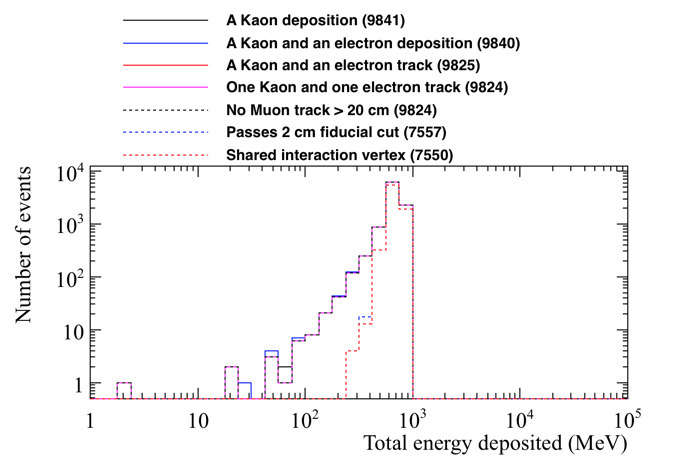
\includegraphics[width=0.8\textwidth]{NucleonDecay_EnergyDepCuts_Raw_2cmCut}
  \caption[The energy distribution of signal events surviving the application of sequential cuts in the $n \rightarrow K^{+} + e^{-}$ channel]
          {The energy distribution of signal events surviving the application of sequential cuts in the $n \rightarrow K^{+} + e^{-}$ channel. The total energy deposited in the detector is plotted on the $x$ axis.}
  \label{fig:NDK_Sig_Raw}
\end{figure}

\begin{figure}
  \centering
  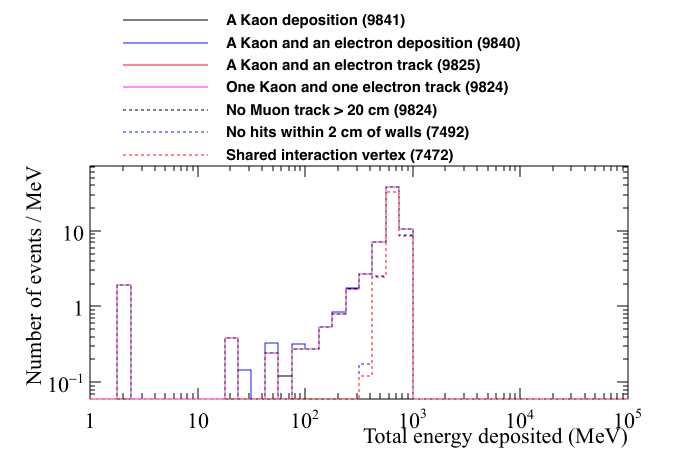
\includegraphics[width=0.8\textwidth]{NucleonDecay_EnergyDepCuts_Norm_2cmCut}
  \caption[The energy distribution of signal events per MeV of deposited energy surviving the application of sequential cuts]
          {The energy distribution of signal events per MeV of deposited energy surviving the application of sequential cuts. The total energy deposited in the detector is plotted on the $x$ axis. This distribution is obtained by dividing the number of events within an energy bin by the bin width.}
  \label{fig:NDK_Sig_Norm}
\end{figure}

When comparing Figures~\ref{fig:NDK_Sig_Raw} and~\ref{fig:NDK_Sig_Norm} with Figures~\ref{fig:NDK_CosmoBack_Raw} and~\ref{fig:NDK_CosmoBack_Norm}, the most obvious difference is that when considering the nucleon decay events, the total energy deposited in the detector never exceeds 1 GeV, whilst in the cosmogenic background sample, the energy deposited in the detector frequently exceeds 1 GeV. This is something which one would expect, as the simulated neutrons decay at rest, and so have a total energy of less than 1 GeV, meaning that there cannot be more than 1 GeV deposited in the detector. This is in stark contrast to the cosmogenic background, where the primary muons being generated have a mean energy of 283 GeV, as shown in Table~\ref{tab:MUSUNflux}. This means that many events will deposit significant amounts of energy in the detector, even if the primary muon misses the detector volume. \\

%%%%% Kaon decay section
A striking feature of Figures~\ref{fig:NDK_Sig_Raw} and~\ref{fig:NDK_Sig_Norm}, is the double peaked structure of the total energy deposited in the detector. This can be attributed to the amount of energy from the kaon decay which is not reconstructed. The relative strengths of these structural features is due to the various probabilities of the kaon decay modes. Some of the more common decay modes are shown in Table~\ref{tab:NDK_KaonDecayRat}, along with their probabilities. The amount of energy which is reconstructed from the particles produced by the decay of the kaon is shown in Figure~\ref{fig:NDK_KaonDecayEn}. \\

\begin{table}
  \caption[The most common decay modes of charged kaons, and their probabilities]
          {The most common decay modes of charged kaons, and their probabilities~\citep{PDGReview}. The decay modes shown are with reference to $K^{+}$, though the decays of $K^{-}$ are the charge conjugations of these decays.}
  \centering
  \label{tab:NDK_KaonDecayRat}
  \begin{tabular}{c c}
    \toprule
        {Decay mode}                                      & {Measured probability (\%)} \\
        \midrule
        $K^{+} \rightarrow \mu^{+} + \nu_{\mu}$           & 63.56 $\pm$ 0.11 \\

        $K^{+} \rightarrow \pi^{+} + \pi^{0}$             & 20.67 $\pm$ 0.08 \\

        $K^{+} \rightarrow \pi^{+} + \pi^{+} + \pi^{-}$   & 5.583 $\pm$ 0.024 \\

        $K^{+} \rightarrow \pi^{0} + e^{+} + \nu_{e}$     & 5.07 $\pm$ 0.04 \\

        $K^{+} \rightarrow \pi^{0} + \mu^{+} + \nu_{\mu}$ & 3.352 $\pm$ 0.033 \\

        $K^{+} \rightarrow \pi^{+} + \pi^{0} + \pi^{0}$   & 1.760 $\pm$ 0.023 \\
        \bottomrule
  \end{tabular}
\end{table}

\begin{figure}
  \centering
  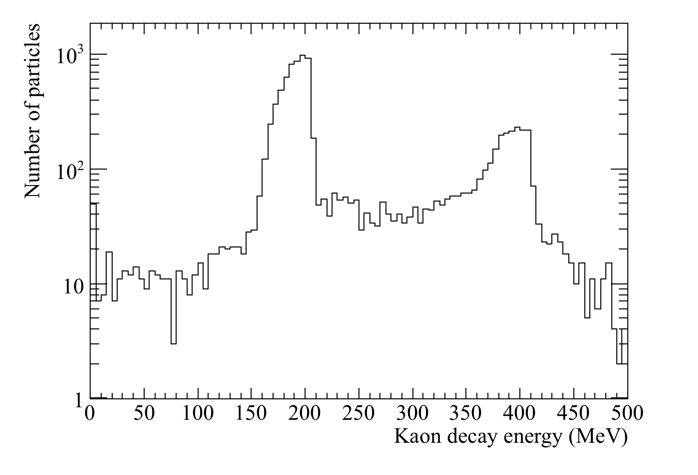
\includegraphics[width=0.8\textwidth]{NucleonDecay_KaonDecayEnergy}
  \caption[The number of events as a function of the energy deposited by the kaon decay products.]
          {The number of events as a function of the energy deposited by the kaon decay products. The energies deposited due to the $K^{+} \rightarrow \mu^{+} + \nu_{\mu}$ and $K^{+} \rightarrow \pi^{+} + \pi^{0}$ decay channels can be seen in the peaks at roughly 200 MeV, and 400 MeV, respectively. The underlying continuous distribution of depositions is caused by the 3-body decays shown in Table~\ref{tab:NDK_KaonDecayRat}.}
  \label{fig:NDK_KaonDecayEn}
\end{figure}

As can be seen in Table~\ref{tab:NDK_KaonDecayRat}, the most common decay mode for the kaon involves the production of a $\nu_{\mu}$, which will leave the detector without interacting. As the kaon is assumed to decay at rest, a significant proportion of the kaon rest mass energy will not be seen. This means that the most likely amount of energy deposited by the kaon decay products is around 200 MeV. The second most likely decay mode is also a 2-body decay, though some of the kaon rest mass energy will not be seen when the $\pi^{+}$ decays. This is why the second peak at 400 MeV is less than the rest mass of the kaon. Neutrinos are also present in many of the other decay modes, and so will also have large amounts of missing energies, whilst the 3-body decay modes will produce particles which have a continuous distribution of energies. These decay modes cause the energy deposited by the kaon decay products to be a continuous distribution, with two large peaks at roughly 200 MeV and 400 MeV, due to the 2 two body decays illustrated above. \\
%%%%% Kaon decay section

The initial cuts, requiring that both a kaon track and an electron shower are observed in the decay, show that there are occasions when either the kaon, or the electron, do not deposit energy in the detector. This affects very few events, though an example of one such event is shown in Figure~\ref{fig:NDK_Sig_MissedKaon}, where it can be seen that the kaon decayed before entering the active volume, and so no track was found for it. It would be very difficult to identify this event as a signal event, as the presence of the kaon could only be inferred from the muon originating from the gap between the APAs, and the energy deposited by the kaon itself will not be reconstructed. Further compounding the identification of this event as a signal event, is the fact that the electron produced in the nucleon decay scatters back into the gap between the APAs. This means that a significant amount of the rest mass energy of the neutron would not be reconstructed. \\

\begin{figure}
  \centering
  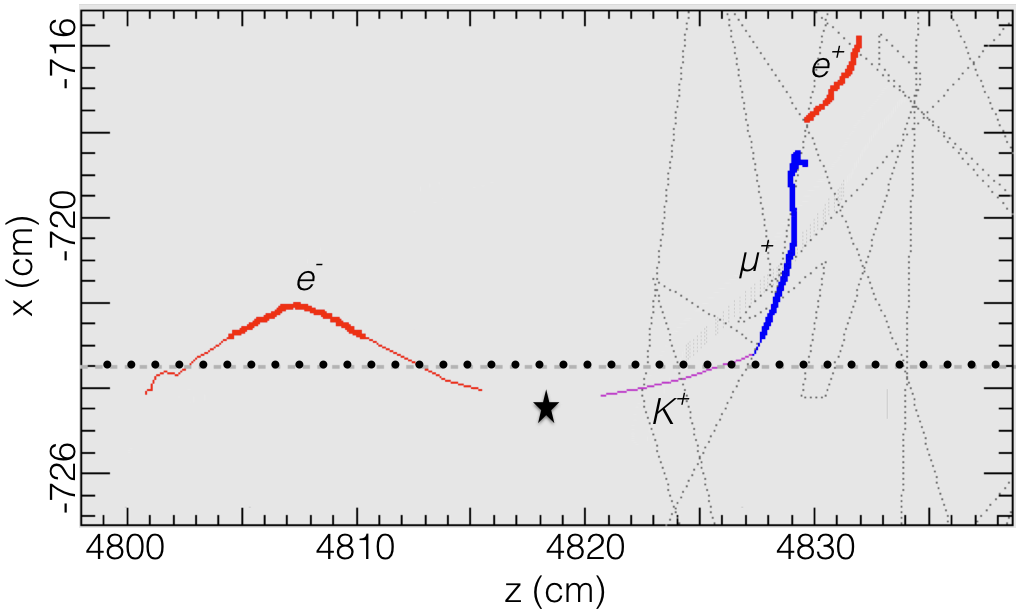
\includegraphics[width=0.8\textwidth]{MissedKaon}
  \caption[A simulated $n \rightarrow K^{+} + e^{-}$ decay where the kaon did not deposit any energy in the active volume]
          {A simulated $n \rightarrow K^{+} + e^{-}$ decay where the kaon did not deposit any energy in the active volume. The path of the kaon produced in the decay is shown as a purple line. The path of the muon, produced by the decay of the kaon, is shown as a blue line. The paths which the electrons in the event took are shown as red lines. The electron on the left of the figure is the electron produced in the neutron decay, whilst the one on the right of the figure, is produced by the decay of the muon. The thin coloured lines show track segments which were in uninstrumented parts of the detector, such as gaps between TPCs and APAs. The dotted black lines show the edges of the TPCs, and the black star shows the location at which the decay occurred. It can be seen that the kaon decayed before it entered the active volume of the detector, and so no track was found for it. A significant portion of the distance which the electron from the decay travelled was also outside the active volume of the detector.}
  \label{fig:NDK_Sig_MissedKaon}
\end{figure}

The number of events which are removed by the fiducial cut is concerning, as when it is considered in conjunction with other cuts, it removes almost 25\% of events. This suggests that the cut is too strict. The reason for this is two fold. Firstly, protons and neutrons are emitted from the nucleus in many of the simulated decays, and whilst the protons produced will create relatively short tracks, which are connected to the decay vertex, the neutrons will travel large distances, and cause energy depositions which are far away from the decay vertex. The faint grey dashed lines, which can be seen in Figure~\ref{fig:NDK_Sig_MissedKaon}, show the spallation neutrons produced in the decay. None of the figures shown here contain spallation protons, but if they were present, they would be shown as additional purple lines originating from the decay vertex. In a large number of events, energy depositions from the spallation neutrons are causing events to fail the ``no energy depositions within 2 cm of the detector edge'' cut by depositing very small of amounts of energy close to the detector walls. Secondly, though the decays are randomly distributed in the active volume of the detector, some of these decays will occur close to the detector walls. For example, over 5\% (25\%) of the neutron decays occur within 30 (100) cm of the detector walls. An example of one such event is shown in Figure~\ref{fig:NDK_Sig_KENearEdge}, where the kaon produced in the decay deposits a significant amount of energy close to the edge of the detector. As a result, it is likely that this cut needs to be relaxed to instead be a cut on the amount of energy deposited within 2 cm of the detector edge. Figure~\ref{fig:NDK_EDepNearEdge} shows the amount of energy deposited within 2 cm, 5 cm, and 10 cm of the detector edges, for the simulated nucleon decay events (Figure~\ref{fig:NDK_EDepNearEdge_Sig}), and the cosmogenic background events (Figure~\ref{fig:NDK_EDepNearEdge_Bk}). \\ 

\begin{figure}
  \centering
  \begin{subfigure}{0.75\textwidth}
    \centering
    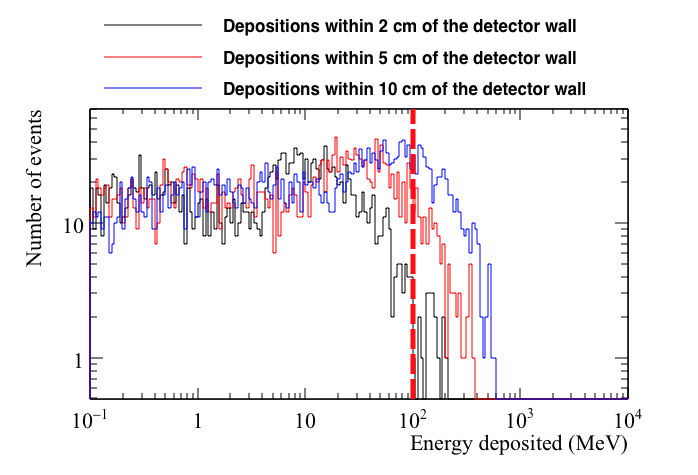
\includegraphics[width=\textwidth]{NucleonDecay_EDepNearEdges}
    \caption{The nucleon decay events.}
    \label{fig:NDK_EDepNearEdge_Sig}
  \end{subfigure}
  % ========
  \begin{subfigure}{0.75\textwidth}
    \centering
    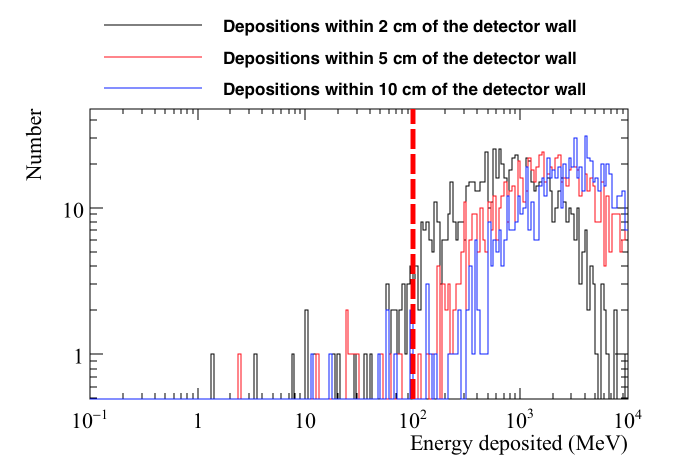
\includegraphics[width=\textwidth]{CosmicBackground_EDepNearEdges}
    \caption{The cosmogenic background events.}
    \label{fig:NDK_EDepNearEdge_Bk}
  \end{subfigure}
  % ========
  \caption[The number of events, as a function of the energy deposited within 2 cm, 5 cm, and 10 cm of the detector edges.]
          {The number of events, as a function of the energy deposited within 2 cm, 5 cm, and 10 cm of the detector edges. Top: energy depositions for the simulated neutron decay events. Bottom: energy depositions for the simulated cosmogenic background events. The histograms are filled after the cut requiring that there is at least one kaon track and at least one electron shower in the event, is applied. As such, the histograms are filled with 9,623 and 1,393 events for the top and bottom histograms respectively. The dashed red line shows the effect of a cut on the energy deposited of 10 MeV. This cut will remove all events which are to the right of the line.}
  \label{fig:NDK_EDepNearEdge}
\end{figure}

As can be seen from Figure~\ref{fig:NDK_EDepNearEdge}, the amount of energy deposited near the detector edges is very different in the nucleon decay sample, and the cosmogenic background sample. As such, they can be relatively cleanly separated. In many of the signal events less than 0.1 MeV of energy is deposited near the detector edge, and so these events are not shown here. It can be seen that in some signal events there are significant energy depositions near the detector edge. Figure~\ref{fig:NDK_Sig_KENearEdge} shows an event where the kaon and electron shower deposit large amounts of energy near the detector edge. The energies deposited near the detector edge by the background events is very large, and is generally due to the presence of large showers which enter the detector. \\

A cut demanding that there should be no more than 10 MeV of energy deposited within 2 cm of the detector edge is used. This cut is designed to preserve as many of the simulated signal events as possible, whilst rejecting as many background events as possible. This cut removes only 683 of the 9,623 signal events, whilst only 39 out of the 1,393 cosmic background events meet this requirement. Whilst this does cause the fiducial cut to become less effective at removing background events from the cosmic sample, it does not cause the huge loss of signal events seen when using the hard cut of ``no energy depositions within 2 cm of the detector edge.'' It is also important to remember that the other cuts will still be applied to these 39 events, as the fiducial cut is not applied in isolation. As will be seen in Figure~\ref{fig:NDK_FidCut_EnLim_Cosmo} none of the muon-induced background events survive the application of all cuts. \\

The definition used to decide if the kaon track and the electron shower share a common vertex seems to be a reasonable requirement, as almost all of the signal events satisfy this definition. Figure~\ref{fig:NDK_Sig_KEDist} shows the distance between the start of the kaon track and the start of the electron shower in signal events. It can be seen that the separation between the two particles is very small (<0.1 cm) in most events. However, there are some events where the separations are very large (>10 cm). As discussed earlier, the decays in these events occur in the gaps between TPCs, such as that shown in Figure~\ref{fig:NDK_Sig_KEBigGap}. When the requirement that the kaon track and the electron shower have a PoCA of less than 2 cm is then applied to these events, most of them are then seen to have a common interaction vertex. For example, this is found to be the case for the event shown in Figure~\ref{fig:NDK_Sig_KEBigGap}. However, in some events the kaon track and the electron shower are still not found to have a common interaction vertex. Hand scanning shows that the particles in these events undergo scattering before entering the active volume, and so by the time that energy depositions occur, their trajectories are no longer closely aligned. This causes the PoCA to be larger than 2 cm, and so they are not identified as a signal event. \\

\begin{figure}
  \centering
  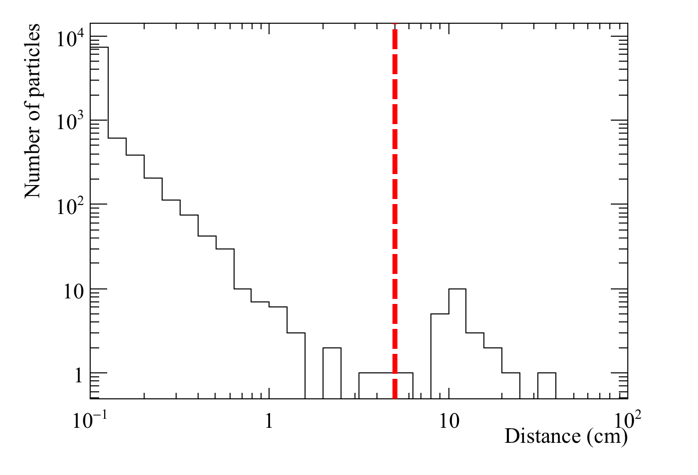
\includegraphics[width=0.8\textwidth]{NucleonDecay_KaonElecSep}
  \caption[The separation of the kaon and the electron produced in the simulated $n \rightarrow K^{+} + e^{-}$ decays]
          {The separation of the kaon and the electron produced in the simulated $n \rightarrow K^{+} + e^{-}$ decays. The dashed red line, drawn at a separation of 5 cm, shows the maximum possible separation a kaon and an electron could have, and still be considered to have a common vertex. A separation of 5 cm is used as this is the separation of the TPCs in the FD. Events with separations of more than this, occur within the centre of an APA.}
  \label{fig:NDK_Sig_KEDist}
\end{figure}

Figure~\ref{fig:NDK_FidCut_EnLim} shows the energy distributions per MeV of deposited energy for the simulated decay (Figure~\ref{fig:NDK_FidCut_EnLim_Sig}) and cosmogenic background (Figure~\ref{fig:NDK_FidCut_EnLim_Cosmo}) events, after the fiducial cut is changed to require that there is less than 10 MeV of energy deposited within 2 cm of the detector edge. As before, these distributions are obtained by dividing the number of events within an energy bin by the bin width. \\

\begin{figure}
  \centering
  \begin{subfigure}{0.8\textwidth}
    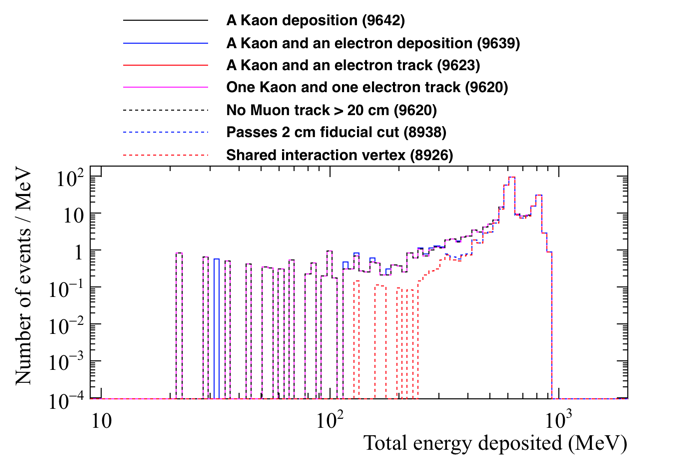
\includegraphics[width=\textwidth]{NucleonDecay_EnergyDepCuts_Norm}
    \caption{The energy distribution of signal events.}
    \label{fig:NDK_FidCut_EnLim_Sig}
  \end{subfigure}
  % ========
  \begin{subfigure}{0.8\textwidth}
    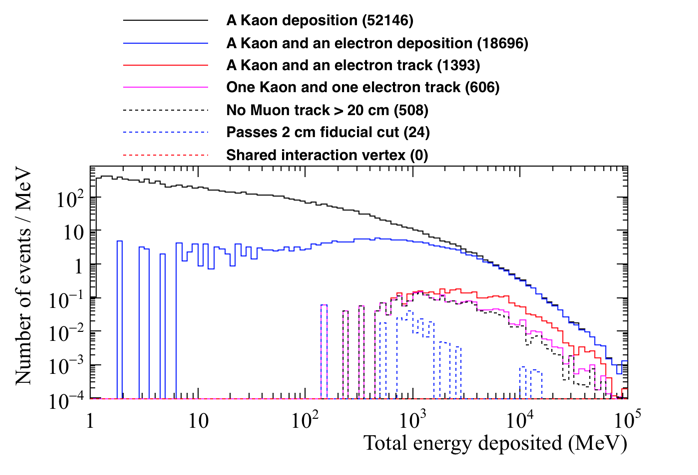
\includegraphics[width=\textwidth]{CosmicBackground_EnergyDepCuts_Norm}
    \caption{The energy distribution of cosmic background events.}
    \label{fig:NDK_FidCut_EnLim_Cosmo}
  \end{subfigure}
  \caption[The energy distributions per MeV of deposited energy for the signal and cosmic background events, surviving the application of sequential cuts after the fiducial cut is modified]
          {The energy distributions per MeV of deposited energy for the signal and cosmic background events, surviving the application of sequential cuts after the fiducial cut is modified. The total energy deposited in the detector is plotted on the $x$ axis. These distributions are obtained by dividing the number of events within an energy bin by the bin width.}
  \label{fig:NDK_FidCut_EnLim}
\end{figure}

The number of signal events which are removed by the cuts can be seen to be much more reasonable after the fiducial cut is modified, as just 1,074 (10.74\%) of the 10,000 signal events are removed as cuts are applied. It is seen that in many of the simulated decay events which fail the cuts, at least one of the kaon, or the electron, are not contained in the active volume of the detector. This means that, either no depositions are found for at least one of the particles (361 events), or there are large energy depositions close to the edge of the detector (683 events). \\

It can be seen that none of the cosmic background events pass the application of all cuts. Of the 24 events which pass the fiducial cut, only 9 of them deposit less than 1 GeV in the detector. This means that the total energy deposited in the detector is usually more than the rest mass of a neutron, and so the event is not consistent with being from the decay of a neutron at rest. Section~\ref{sec:NDKEnCosmBk} will consider the energy deposition distributions of the simulated neutron decay events, though it is first necessary to calculate the expected values of these energy depositions, this is shown in Section~\ref{sec:NDKKin}. \\

%********************************** % Third Section  *************************************
\subsection{Kinematics of nucleon decay} \label{sec:NDKKin}
It is possible to apply strict energy criteria to the reconstructed energies of candidate nucleon decay events, as the distributions which one would expect are well defined. When determining the kinematics of the $n \rightarrow K^{+} e^{-}$ decay channel, the neutron is assumed to decay at rest. The resulting kinematic equations are presented below:
\begin{align}
  E_{n} &= m_{n} = E_{K} + E_{e} \nonumber \\
  E_{e}^{2} &= (m_{n} - E_{K})^{2} \nonumber \\
  m_{e}^{2} + p_{e}^{2} &= m_{n}^{2} + (m_{K}^{2} + p_{K}^{2}) - 2m_{n}E_{K} \nonumber \\
  &\text{using conservation of momentum $\vec{p}_{K} = -\vec{p}_{e}$} \nonumber \\  
  E_{K} &= \frac{m_n^{2} + m_{K}^{2} - m_{e}^{2}}{2m_{n}} \label{eq:DecKEn} \\
  E_{e} &= \frac{m_n^{2} + m_{e}^{2} - m_{K}^{2}}{2m_{n}} \label{eq:DecEEn} \\
  \sqrt{E_{K}^{2} - m_{K}^{2}} = \vec{p_{K}} &= \sqrt{ \left(\frac{m_n^{2} + m_{e}^{2} - m_{K}^{2}}{2m_{n}}\right)^{2} - m_{K}^{2}\left(\frac{4m_{n}^2}{4m_n^{2}}\right) } \nonumber \\
  \vec{p_{K}} &= \frac{ \sqrt{m_n^{2} + m_{K}^{2} - m_{e}^{2} - 4m_{n}^{2}m_{K}^{2} } }{ 2m_{n} } \label{eq:DecEMom} \\
  \vec{p_{e}} &= \frac{ \sqrt{m_n^{2} + m_{e}^{2} - m_{K}^{2} - 4m_{n}^{2}m_{e}^{2} } }{ 2m_{n} } \label{eq:DecKMom}
\end{align}
Using $m_{n}$ = 939.565 MeV, $m_{K}$ = 493.677 MeV and $m_{e}$ = 0.511 MeV~\citep{PDGReview}, the total kaon and electron energies are equal to 599.479 MeV and 340.086 MeV respectively, whilst the momenta of the kaon and electron are both equal to 340.086 MeV. A kaon (electron) with total energy $E_{K}$ = 599.479 ($E_{e}$ = 340.086) MeV will have a kinetic energy of 105.802 (339.575) MeV. \\

It is important to note that any nucleon which decays in LArTPCs will be contained in argon nuclei, this means that the energies of any particles which are produced will be smeared by the Fermi motion of the decaying nucleon within the nucleus. Any kaon which is produced in the decay is also likely to scatter as it exits the nucleus, further smearing its energy and momenta~\citep{Stefan:2008zi}. This causes the true momenta and total energy of the particles produced in the decay to be different from the values which were calculated above. Thus, when searching for nucleon decay events, it is necessary to consider energy ranges of a few hundred MeV. This also takes into account the energy resolution of the detector. \\

%********************************** % Fifth.Second Section  *************************************
\subsection{Energy constraints on the cosmogenic background to the $n \rightarrow K^{+} + e^{-}$ decay channel} \label{sec:NDKEnCosmBk}
As outlined in Section~\ref{sec:NDKCosmBk}, it is possible to exclude background events from signal events using the distribution of energy depositions in the detector. As previously outlined, the energy depositions were split into several categories:
\begin{itemize}
\item The energy directly deposited by the kaon and its secondaries, excluding its decay products.
\item The energy deposited by the kaon decay products and any of their secondaries.
\item The energy directly deposited by the electron and its secondaries.
\item The energy deposited near the shared kaon and electron vertex that is not associated with the kaon or electron.
\item The energy deposited in the detector which does not fit any of the above criteria.
\end{itemize}
Following the earlier discussions in Section~\ref{sec:NDKCosmBk}, it should be clear that the energy directly deposited by the kaon corresponds to the sum of all energy depositions, which are due to the kaon or its interaction products. Equivalently, the energy directly deposited by the electron, corresponds to the sum of all energy depositions which are due to the electron as it showers, and any particles created as a result of the shower. The energy deposited by the kaon decay products would include all depositions by the muon and subsequent electron, in the case that the kaon decayed via $K^{+} \rightarrow \mu^{+} + \nu_{\mu}$, and then the muon decayed via $\mu^{+} \rightarrow e^{+} + \nu_{e} + \overline{\nu_{\mu}}$. The energy deposited near the shared kaon and electron vertex, would primarily consist of energy depositions due to spallation products. These depositions would largely be due to protons, though may also include some depositions due to neutrons too, if they deposited energy near the interaction vertex. Any depositions within 5 cm of either the start of the kaon track, or the start of the electron shower, are considered ``near'' to the interaction vertex. It is necessary to consider the energy depositions which are close to the start of both particles, because occasionally the particles are separated by the APA gaps, as shown in Figure~\ref{fig:NDK_Sig_KEBigGap}. As can be seen from Figure~\ref{fig:NDK_Sig_KEDist}, the separation between the start of the kaon track and the start of the electron shower, is normally very small. This means that the sum of the ``near'' energy depositions, can be considered to be the energy depositions ``near'' the common vertex between the kaon track and the electron shower. The final criteria, of any depositions which do not fit the above description, would largely consist of energy depositions due to the spallation neutrons in the decay sample. However, in the cosmic background sample, this would include all depositions by muons, pions, and any other particles in the detector which are not associated with either the kaon or the electron. In later discussions these depositions are generally referred to as ``other'' energy depositions. \\

In presenting the separation of simulated cosmic background events and simulated neutron decay events, the important distributions to consider are as follows:
\begin{itemize}
\item The energy directly deposited by the kaon, against the energy directly deposited by the electron. This is shown in Figure~\ref{fig:NDK_Kaon_Elec_EDist}.
\item The energy directly deposited by the kaon, plus the energy directly deposited by the electron, against the energy deposited near the shared kaon and electron vertex. This is shown in Figure~\ref{fig:NDK_KaonElec_Near_EDist}.
\item The energy deposited by the kaon, including decay products, against the energy deposited in the detector which does not fit any of the other criteria. This is shown in Figure~\ref{fig:NDK_AllKaon_Other_EDist}.
\item The energy deposited by the kaon, including decay products, plus the energy directly deposited by the electron, plus the energy deposited near the shared kaon and electron vertex, against the energy deposited in the detector which does not fit any of the other criteria. This is shown in Figure~\ref{fig:NDK_AllEDep_Other_EDist}.
\end{itemize}
Each of these figures will be discussed in turn below. The events in the nucleon decay sample which pass all cuts have been plotted with smaller markers, this is to allow the less numerous events which fail the cuts to be visible. \\

Additionally, the figures outlined above have a box in the lower left corner of the plots produced by dashed grey lines. This constitutes the expected energy region where a signal event would lie on the graph, and has been drawn so as to contain as many of the simulated signal events as possible. The expected energy regions are propagated down to 0 MeV on both the $x$ and $y$ axis of all figures, and so it is possible for points not drawn here to pass the applied cuts. This is because it is possible for signal events to have no energy identified as ``near'' the common interaction vertex, such as the event shown in Figure~\ref{fig:NDK_Sig_KEBigGap}. It is also possible for there to be no energy deposition which would be classed as ``other'' energy depositions. \\

% ========== Kaon vs Elec
\begin{figure}
  \centering
  \begin{subfigure}{0.8\textwidth}
    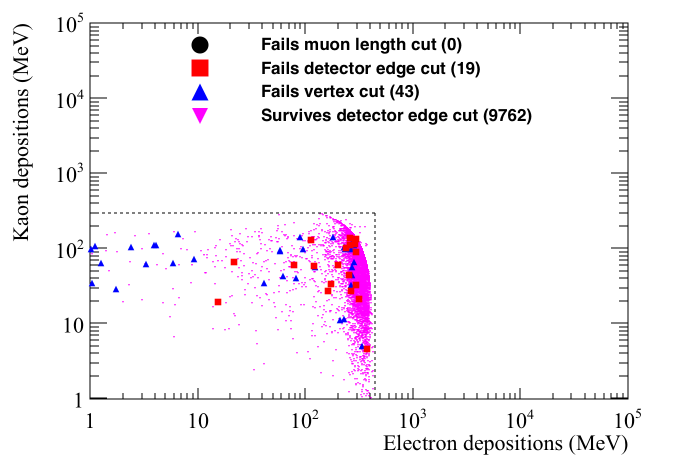
\includegraphics[width=\textwidth]{NucleonDecay_Kaon_vs_Elec_Can}
    \caption{Signal events.}
    \label{fig:NDK_Kaon_Elec_EDist_Sig}
  \end{subfigure}
  % ========
  \begin{subfigure}{0.8\textwidth}
    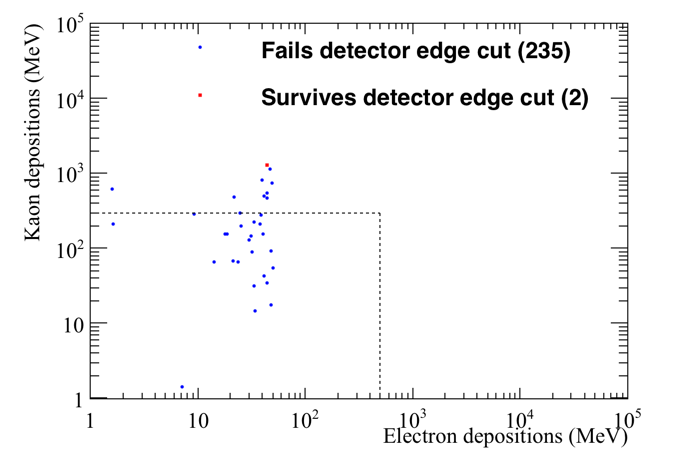
\includegraphics[width=\textwidth]{CosmicBackground_Kaon_vs_Elec_Can}
    \caption{Cosmic background events.}
    \label{fig:NDK_Kaon_Elec_EDist_Cosmo}
  \end{subfigure}
  \caption[The energy directly deposited by kaons versus the energy directly deposited by electrons, in the simulated nucleon decay and cosmic background samples]
          {The energy directly deposited by kaons versus the energy directly deposited by electrons, in the simulated nucleon decay (top) and cosmic background samples (bottom). The events failing the application of the muon length (black circle), fiducial (green box) and vertex (blue triangle) cuts, as well as the events passing all cuts (red triangle) are shown. The cuts are those defined at the start of Section~\ref{sec:NDKCosmBk}.}
  \label{fig:NDK_Kaon_Elec_EDist}
\end{figure}

% ========== Kaon + Elec vs Near
\begin{figure}
  \centering
  \begin{subfigure}{0.8\textwidth}
    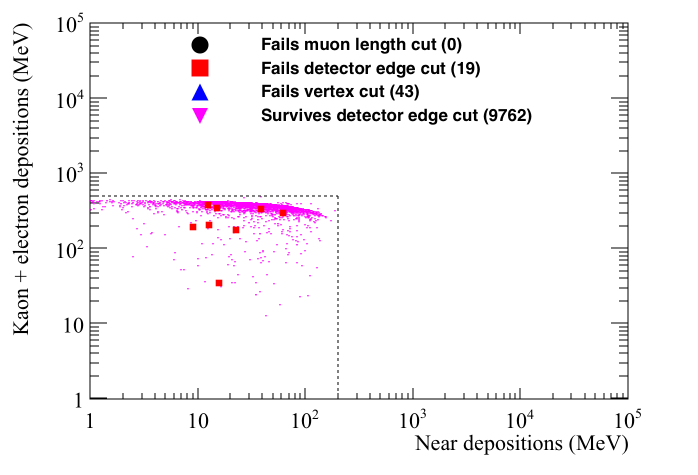
\includegraphics[width=\textwidth]{NucleonDecay_KaonElec_vs_Near_Can}
    \caption{Signal events.}
    \label{fig:NDK_KaonElec_Near_EDist_Sig}
  \end{subfigure}
  % ========
  \begin{subfigure}{0.8\textwidth}
    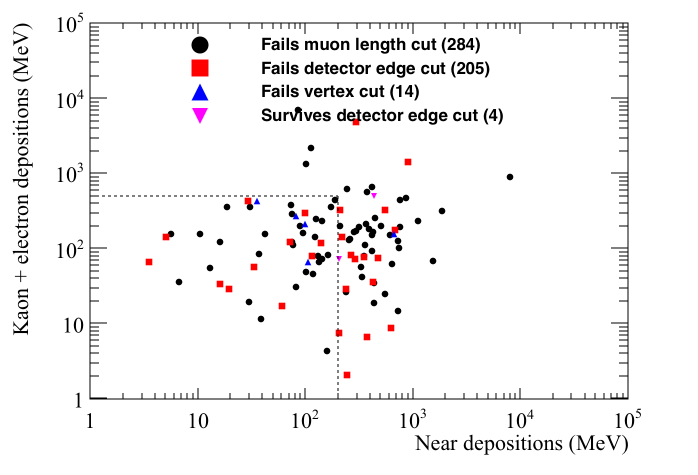
\includegraphics[width=\textwidth]{CosmicBackground_KaonElec_vs_Near_Can}
    \caption{Cosmic background events.}
    \label{fig:NDK_KaonElec_Near_EDist_Cosmo}
  \end{subfigure}
  \caption[The energy directly deposited by kaons, plus the energy directly deposited by electrons versus the energy deposited near the kaon and electron vertex, in the simulated nucleon decay and cosmic background samples]
          {The energy directly deposited by kaons, plus the energy directly deposited by electrons versus the energy deposited near the kaon and electron vertex, in the simulated nucleon decay (top) and cosmic background samples (bottom). The events failing the application of the muon length (black circle), fiducial (green box) and vertex (blue triangle) cuts, as well as the events passing all cuts (red triangle) are shown. The cuts are those defined at the start of Section~\ref{sec:NDKCosmBk}.}
  \label{fig:NDK_KaonElec_Near_EDist}
\end{figure}

% ========== Kaon + Kaon Decay vs Other
\begin{figure}
  \centering
  \begin{subfigure}{0.8\textwidth}
    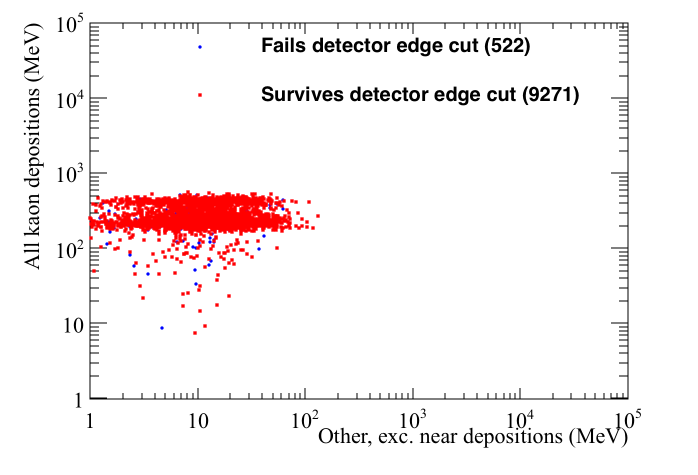
\includegraphics[width=\textwidth]{NucleonDecay_AllKaon_vs_Other_Can}
    \caption{Signal events.}
    \label{fig:NDK_AllKaon_Other_EDist_Sig}
  \end{subfigure}
  % ========
  \begin{subfigure}{0.8\textwidth}
    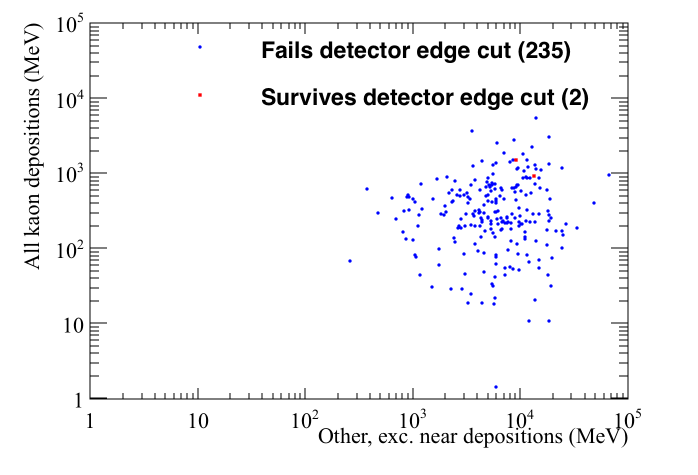
\includegraphics[width=\textwidth]{CosmicBackground_AllKaon_vs_Other_Can}
    \caption{Cosmic background events.}
    \label{fig:NDK_AllKaon_Other_EDist_Cosmo}
  \end{subfigure}
  \caption[The energy directly deposited by kaons, plus the energy deposited by the kaon decay products versus the energy depositions which do not fit any of the other criteria, in the simulated nucleon decay and cosmic background samples]
          {The energy directly deposited by kaons, plus the energy deposited by the kaon decay products versus the energy depositions which do not fit any of the other criteria, in the simulated nucleon decay (top), and cosmic background samples (bottom). The events failing the application of the muon length (black circle), fiducial (green box) and vertex (blue triangle) cuts, as well as the events passing all cuts (red triangle) are shown. The cuts are those defined at the start of Section~\ref{sec:NDKCosmBk}.}
  \label{fig:NDK_AllKaon_Other_EDist}
\end{figure}

% ========== Kaon + Kaon Decay + Elec + Near vs Other
\begin{figure}
  \centering
  \begin{subfigure}{0.8\textwidth}
    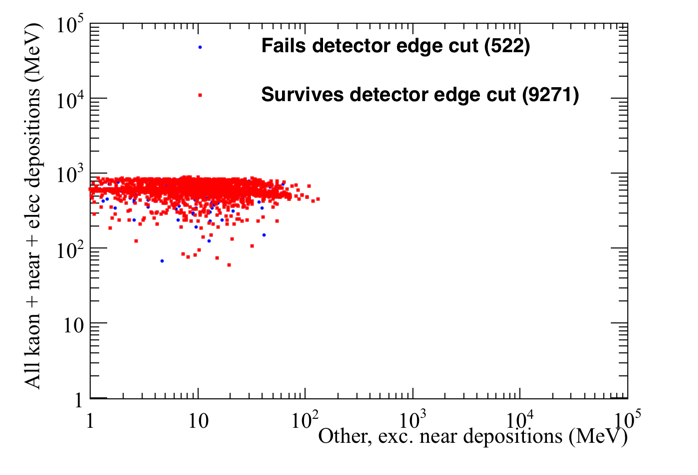
\includegraphics[width=\textwidth]{NucleonDecay_AllKaonNearElec_vs_Other_Can}
    \caption{Signal events.}
    \label{fig:NDK_AllEDep_Other_EDist_Sig}
  \end{subfigure}
  % ========
  \begin{subfigure}{0.8\textwidth}
    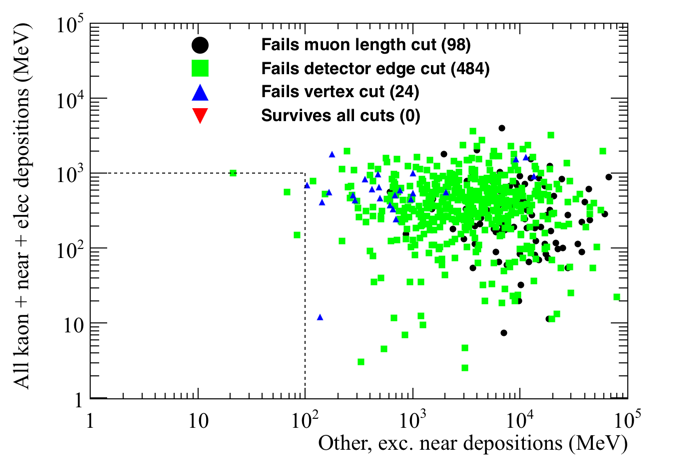
\includegraphics[width=\textwidth]{CosmicBackground_AllKaonNearElec_vs_Other_Can}
    \caption{Cosmic background events.}
    \label{fig:NDK_AllEDep_Other_EDist_Cosmo}
  \end{subfigure}
  \caption[The energy directly deposited by kaons, plus the energy deposited by the kaon decay products, plus the energy directly deposited by electrons, plus the energy deposited near the kaon and electron vertex versus the energy depositions which do not fit any of the other criteria, in the simulated nucleon decay and cosmic background samples]
          {The energy directly deposited by kaons, plus the energy deposited by the kaon decay products, plus the energy directly deposited by electrons, plus the energy deposited near the kaon and electron vertex versus the energy depositions which do not fit any of the other criteria, in the simulated nucleon decay (top) and cosmic background samples (bottom). The events failing the application of the muon length (black circle), fiducial (green box) and vertex (blue triangle) cuts, as well as the events passing all cuts (red triangle) are shown. The cuts are those defined at the start of Section~\ref{sec:NDKCosmBk}.}
  \label{fig:NDK_AllEDep_Other_EDist}
\end{figure}

% ========== Kaon vs Elec
From Figure~\ref{fig:NDK_Kaon_Elec_EDist}, it can be seen that the electron energy distribution in the cosmic background sample, is very different from the one seen in the simulated neutron decay sample. The energies deposited by electrons in the nucleon decay sample are tightly concentrated between $\sim$200 and $\sim$400 MeV, whilst in the cosmic background sample, the energy deposited by the electron is almost always less than $\sim$50 MeV. Many of the electrons in the cosmic background sample deposit less than 1 MeV of energy in the detector, and so are not shown in Figure~\ref{fig:NDK_Kaon_Elec_EDist_Cosmo}. This is why Figure~\ref{fig:NDK_Kaon_Elec_EDist_Cosmo} is very sparse despite 606 events being plotted. Realistically, these electrons are unlikely to be reconstructed due to their extremely low energies. From Figure~\ref{fig:NDK_Kaon_Elec_EDist_Sig}, it can be seen that some of the electrons produced in the nucleon decay events also deposit very little energy in the detector, though these events generally fail either the fiducial cut, or the vertex cut. An explanation as to why these events fail the cuts was presented in Section~\ref{sec:NDKSig}, when considering Figure~\ref{fig:NDK_Sig_MissedKaon}. \\

% ========== Kaon + Elec vs Near
From Figure~\ref{fig:NDK_KaonElec_Near_EDist_Sig}, it can be seen that as the energy deposited near the kaon and electron vertex increases, the sum of the energy deposited by the kaon and electron decreases. This is reasonable, because, when the spallation protons and neutrons have more energy, the kaon and electron will have less energy. The decrease in the energy deposited by the kaon and the electron, is roughly consistent with the increase in the amount of energy which is deposited near their shared vertex. This means that the sum of the three energies is generally around 450 MeV, as expected from the kinematic calculations shown in Section~\ref{sec:NDKKin} where a two body decay was assumed. Though this is no longer valid when 3+ particles are produced, the majority of the rest mass energy of the neutron will be still be measured if the neutron energies are small. This is largely inconsistent with the simulated cosmic background events, where many events have no energy deposited near the shared vertex of the kaon and electron. However, the lack of energy deposited near the shared kaon and electron vertex cannot be used to discriminate against cosmogenic background events, as this is also observed in many simulated nucleon decay events. What can be used to separate cosmic background events from nucleon decay events though, is the sum of the three energy criteria, as it can be seen that this would rarely be around 450 MeV in the cosmic background sample. \\

% ========== Kaon + Kaon Decay vs Other
Figure~\ref{fig:NDK_AllKaon_Other_EDist} shows that the sum of all energy deposits attributed to the kaon, against the sum of all energy depositions which are considered to be ``other'' energy depositions, is very different in the two samples. The total energy deposited in the detector which is attributed to the kaon is found by combining the energy directly deposited by the kaon, with the energy deposited by the kaon decay products. This sum is seen to have a banded structure in Figure~\ref{fig:NDK_AllKaon_Other_EDist_Sig}, this is due to the amount of energy from the kaon decay which is not reconstructed, and was discussed when considering Figure~\ref{fig:NDK_KaonDecayEn}. The difference seen in the cosmogenic background and signal events, is primarily due to the large amount of ``other'' energy depositions which are seen in the cosmogenic background sample. This is expected, as in muon-induced events many particles may enter the detector, causing energy depositions which are not connected to the kaon track, the electron shower, or their common vertex, should one exist. This gives the most powerful mechanism for the discrimination between signal and background events, as in many background events the ``other'' energy deposited in the detector will be very large, and will cause the total energy deposited in the detector to be more than the rest mass of a neutron. Also, the ``other'' energy deposited by background events in the detector, will likely be concentrated in track or shower like structures. This is in contrast to signal events, where the ``other'' energy depositions are likely to be isolated depositions due to the spallation neutrons interacting in the detector. Classifying the structure of the ``other'' energy depositions is not performed here, though it could be included should any cosmic events appear to mimic a signal event. However, given the clear separation in the amount of ``other'' energy deposited in the detector, it is not currently required. \\

% ========== Kaon + Kaon Decay + Elec + Near vs Other
Figure~\ref{fig:NDK_AllEDep_Other_EDist} shows the total energy attributed to both the kaon and to the electron, plus any energy deposited near their shared interaction vertex, versus any ``other'' energy depositions. Here, the total energy attributed to the kaon is plotted, including the energy deposited by the kaon decay products, as was the case in Figure~\ref{fig:NDK_AllKaon_Other_EDist}. As was seen in Figure~\ref{fig:NDK_AllKaon_Other_EDist}, there is a clear separation between the simulated signal events, and the cosmic background events. This is again due to the large amount of ``other'' energy depositions observed in the background sample. It is interesting to compare Figures~\ref{fig:NDK_AllKaon_Other_EDist_Cosmo} and~\ref{fig:NDK_AllEDep_Other_EDist_Cosmo}, as they are very similar. This is to be expected from Figure~\ref{fig:NDK_Kaon_Elec_EDist_Cosmo}, where it was seen that the energy deposited by the electron was rarely more than 10 MeV, and was never more than 100 MeV. This was in stark contrast to Figure~\ref{fig:NDK_Kaon_Elec_EDist_Sig}, where the energy deposited in almost all of the electron showers was more than 100 MeV. Hence, whilst there is a large difference in the energy plotted on the $y$ axis of Figures~\ref{fig:NDK_AllKaon_Other_EDist_Sig} and~\ref{fig:NDK_AllEDep_Other_EDist_Sig}, due to the addition of significant energy depositions from the electron showers, there is relatively little difference the energy plotted on the $y$ axis of Figures~\ref{fig:NDK_AllKaon_Other_EDist_Cosmo} and~\ref{fig:NDK_AllEDep_Other_EDist_Cosmo}. \\

A significant difference between Figures~~\ref{fig:NDK_AllKaon_Other_EDist_Sig} and~\ref{fig:NDK_AllEDep_Other_EDist_Sig}, is the relatively narrow band of energies plotted on the $y$ axis of Figure~\ref{fig:NDK_AllEDep_Other_EDist_Sig}, when compared to Figure~\ref{fig:NDK_AllKaon_Other_EDist_Sig}. This is because of the relationship between the energy deposited by the kaon, the energy deposited by the electron shower, and the energy deposited near their shared interaction vertex. This was seen in Figure~\ref{fig:NDK_KaonElec_Near_EDist_Sig}, where the sum of the three energies was roughly 450 MeV. This means that for events where the kaon deposited relatively little energy, shown by the population of events at low total kaon energies in Figure~\ref{fig:NDK_AllKaon_Other_EDist_Sig}, the energy deposited by the electron shower, plus the energy deposited near the shared interaction vertex, will be large. \\

Following the application of all energy cuts, as outlined by the grey dashed boxes in Figures~\ref{fig:NDK_Kaon_Elec_EDist},~\ref{fig:NDK_KaonElec_Near_EDist},~\ref{fig:NDK_AllKaon_Other_EDist}, and~\ref{fig:NDK_AllEDep_Other_EDist}, only 24 of the 8,926 simulated signal events, which passed all subsequent cuts, are removed. If only the energy cuts, and the requirement that there be at least one kaon track, and at least one electron shower in the event, are applied, it is found that only 2 background candidates would survive the application of cuts. None of these events present serious contenders for signal events though, as they both fail the vertex and fiducial cuts, and have electrons which have very little energy (< 10 MeV). \\

Many of the signal events which are removed by the energy cuts have large amounts of ``other'' energy depositions, though they would no longer be removed if the limit on ``other'' depositions were raised to 200 MeV, as seen in Figure~\ref{fig:NDK_AllEDep_Other_EDist_Sig}. Though increasing the cut on ``other'' energy depositions to 200 MeV would still result in all background events being removed, it would mean that the limit was much closer to the regions of ``other'' energy depositions which are populated in Figures~\ref{fig:NDK_AllKaon_Other_EDist_Cosmo}, and~\ref{fig:NDK_AllEDep_Other_EDist_Cosmo}. As a result if a candidate event were to have between 100 and 200 MeV of energy depositions considered to be ``other'' energy depositions, its energy distributions would have to be carefully checked in order to verify that it is definitively not due to a background event. It is envisioned that the process by which this would be done, would be to consider how the ``other'' energy deposits are distributed in the detector. As discussed earlier, in a signal event it is likely that they would be isolated depositions, whereas in a background event, there would likely be ``track-like'' objects disconnected from the kaon and electron vertex. \\

Therefore, the result of a preliminary study on background rejection for the $n \rightarrow K^{+} + e^{-}$ decay channel, found no muon-induced background events which would survive the application of cuts, in a sample of 2 $\times$ 10$^9$ muons representing 401.6 years of detector for a single FD module. This corresponds to a limit of the background rate of less than 0.44~events$\cdot$Mt$^{-1}\cdot$year$^{-1}$ at the 90\% confidence level, using double sided errors~\citep{PDGReview} and a fiducial mass of 13.8~kt to give an exposure of 5.542~Mt$\cdot$year. \\

Using the cuts outlined above, only 10.98\% of signal events are removed, representing a high signal efficiency of 89.02\%, where almost all of the signals which are removed due to at least one of the particles produced in the decay escaping the detector. When only particles which are fully contained in the active volume of the detector are considered, the signal efficiency increases to 96.8\%, where the 2 cm fiducial cut has removed most of the 3.2\% of rejected signal events. These events have particles which travel close to the edge of the detector but do not quite leave it. For example, if the event shown in Figure~\ref{fig:NDK_EDepNearEdge} was a few cm further away from the edge of the detector, then this would be an example of an event which is fully contained in the detector but is rejected by the fiducial cut. If it is apparent that a candidate event is contained in the detector, even though it deposits significant amounts of energy near the detector edge, it may be possible to identify it as a neutron decay, due to the lack of signal mimicking background events which were observed in this study. Therefore, it may be possible to increase the signal efficiencies quoted above by relaxing the 2 cm fiducial cut, though considering events where particles leave the active volume of the detector will mean that PID is more difficult, and the reconstructed energy may be much less than the rest mass of the neutron. \\ 

%********************************** % Fifth.Third Section  *************************************
\subsection{Future improvements to nucleon decay studies and conclusions} \label{sec:NDKImprov}
Thus far, the study of the background to nucleon decay has only focused on the muon-induced background. However, as was mentioned in Section~\ref{sec:BkNDK} atmospheric neutrinos are also able to produce signal mimicking events in underground detectors. There have been no studies to date concerning the atmospheric background to the $n \rightarrow K^{+} + e^{-}$ decay channel, though this will need to be performed before a full background estimation can be made for this decay channel. However, this is a separate study which will have to be performed at a later date. \\

The study of muon-induced background to nucleon decay presented in this thesis has only been performed on Monte Carlo truth information, and so has not used reconstructed objects. The extension of the analysis to include work on tracks is an important next step, as then the full analysis which would be applied to real data can be tested. Preliminary studies have begun on hit reconstruction, and involve running a filter on the muons used in the earlier analyses. This is because the number of events which are saved to disk would be prohibitive to running the full reconstruction process. As such, only events which meet the following criteria will be reconstructed~\citep{CosmoJanCollabMeeting};
\begin{itemize}
\item A minimum of 10 MeV deposited in the detector volume.
\item A maximum of 3,000 MeV deposited in the detector volume.
\item A maximum of 5 MeV deposited within 10 cm of the detector edge.
\end{itemize}
These criteria are designed to be soft enough that the full range of nucleon decay modes can be studied, including di-nucleon decay modes and neutron-antineutron oscillations. This is why the maximum deposited energy greatly exceeds the rest mass of a single nucleon. This also accounts for the fact that during reconstruction some energy depositions may not be reconstructed, so even though the total energy deposited in the detector is 3 GeV, the total reconstructed energy may be less. \\

Upon performing reconstruction, and hence energy and position smearing, it is likely that the energy cuts which were outlined in Section~\ref{sec:NDKEnCosmBk} will have to be broadened. This may result in more background events being contained within the expected energy distributions for signal events, however the effectiveness of the other cuts to remove background events should be largely unaffected. The reason for this is that upon performing reconstruction, the separation of the kaon and electron track will not decrease, and so the cut is expected to remain very efficient. The only cut which may be less effective is the requirement that there only be one kaon track, and only one electron shower in the event. This is because some of the low energy electron showers may not be reconstructed. However, even when this cut was relaxed no background events survived the application of all cuts. \\

The reduced reconstruction efficiency will also affect the nucleon decay signals. This, combined with the broader distributions of energies which will be reconstructed, will mean that the efficiency with which signal events can be identified will probably decrease. Studies have been performed to establish the event identification efficiencies when using reconstructed objects~\citep{KevinSeptCollab, AAron_17_02_08, Tingjun_17_02_08, Aaron_17_03_01}, though currently these have only been done with respect to the $p \rightarrow K^{+} + \overline{\nu_{e}}$ decay channel. These studies have found that the current signal reconstruction efficiency is less than the 100\% assumed here~\citep{AAron_17_02_08}, though it is imagined that this will improve significantly with new releases of the reconstruction software. \\

However, it is envisioned that there will still be no muon-induced background events which survive the application of all cuts, though the impact of atmospheric neutrinos remains to be seen, and so the observation of a single event in the DUNE detector could provide a robust indication of nucleon decay. \\
